%%%%%%%%%%%%%%%%%%%%%%%%%%%%%%%%%%%%%%%%%%
% The Legrand Orange Book
% LaTeX Template
% Version 2.4 (26/09/2018)
%
% This template was downloaded from:
% http://www.LaTeXTemplates.com
%
% Original author:
% Mathias Legrand (legrand.mathias@gmail.com) with modifications by:
% Vel (vel@latextemplates.com)
%
% License:
% CC BY-NC-SA 3.0 (http://creativecommons.org/licenses/by-nc-sa/3.0/)
%
% Compiling this template:
% This template uses biber for its bibliography and makeindex for its index.
% When you first open the template, compile it from the command line with the 
% commands below to make sure your LaTeX distribution is configured correctly:
%
% 1) pdflatex main
% 2) makeindex main.idx -s StyleInd.ist
% 3) biber main
% 4) pdflatex main x 2
%
% After this, when you wish to update the bibliography/index use the appropriate
% command above and make sure to compile with pdflatex several times 
% afterwards to propagate your changes to the document.
%
% This template also uses a number of packages which may need to be
% updated to the newest versions for the template to compile. It is strongly
% recommended you update your LaTeX distribution if you have any
% compilation errors.
%
% Important note:
% Chapter heading images should have a 2:1 width:height ratio,
% e.g. 920px width and 460px height.
%
%%%%%%%%%%%%%%%%%%%%%%%%%%%%%%%%%%%%%%%%%

%----------------------------------------------------------------------------------------
%	PACKAGES AND OTHER DOCUMENT CONFIGURATIONS
%----------------------------------------------------------------------------------------

\documentclass[11pt,fleqn]{book} % Default font size and left-justified equations

%%%%%%%%%%%%%%%%%%%%%%%%%%%%%%%%%%%%%%%%%
% The Legrand Orange Book
% Structural Definitions File
% Version 2.1 (26/09/2018)
%
% Original author:
% Mathias Legrand (legrand.mathias@gmail.com) with modifications by:
% Vel (vel@latextemplates.com)
% 
% This file was downloaded from:
% http://www.LaTeXTemplates.com
%
% License:
% CC BY-NC-SA 3.0 (http://creativecommons.org/licenses/by-nc-sa/3.0/)
%
%%%%%%%%%%%%%%%%%%%%%%%%%%%%%%%%%%%%%%%%%

%----------------------------------------------------------------------------------------
%	VARIOUS REQUIRED PACKAGES AND CONFIGURATIONS
%----------------------------------------------------------------------------------------

\usepackage{graphicx} % Required for including pictures
\graphicspath{{figures/}} % Specifies the directory where pictures are stored

\usepackage{lipsum} % Inserts dummy text

\usepackage{tikz} % Required for drawing custom shapes

\usepackage[english]{babel} % English language/hyphenation

\usepackage{enumitem} % Customize lists
\setlist{nolistsep} % Reduce spacing between bullet points and numbered lists

\usepackage{booktabs} % Required for nicer horizontal rules in tables

\usepackage{xcolor} % Required for specifying colors by name
\definecolor{ocre}{RGB}{243,102,25} % Define the orange color used for highlighting throughout the book

%----------------------------------------------------------------------------------------
%	MARGINS
%----------------------------------------------------------------------------------------

\usepackage{geometry} % Required for adjusting page dimensions and margins

\geometry{
	paper=a4paper, % Paper size, change to letterpaper for US letter size
	top=3cm, % Top margin
	bottom=3cm, % Bottom margin
	left=3cm, % Left margin
	right=3cm, % Right margin
	headheight=14pt, % Header height
	footskip=1.4cm, % Space from the bottom margin to the baseline of the footer
	headsep=10pt, % Space from the top margin to the baseline of the header
	%showframe, % Uncomment to show how the type block is set on the page
}

%----------------------------------------------------------------------------------------
%	FONTS
%----------------------------------------------------------------------------------------

\usepackage{avant} % Use the Avantgarde font for headings
%\usepackage{times} % Use the Times font for headings
\usepackage{mathptmx} % Use the Adobe Times Roman as the default text font together with math symbols from the Sym­bol, Chancery and Com­puter Modern fonts

\usepackage{microtype} % Slightly tweak font spacing for aesthetics
\usepackage[utf8]{inputenc} % Required for including letters with accents
\usepackage[T1]{fontenc} % Use 8-bit encoding that has 256 glyphs

%----------------------------------------------------------------------------------------
%	BIBLIOGRAPHY AND INDEX
%----------------------------------------------------------------------------------------

\usepackage[style=numeric,citestyle=numeric,sorting=nyt,sortcites=true,autopunct=true,babel=hyphen,hyperref=true,abbreviate=false,backref=true,backend=biber]{biblatex}
\addbibresource{bibliography.bib} % BibTeX bibliography file
\defbibheading{bibempty}{}

\usepackage{calc} % For simpler calculation - used for spacing the index letter headings correctly
\usepackage{makeidx} % Required to make an index
\makeindex % Tells LaTeX to create the files required for indexing

%----------------------------------------------------------------------------------------
%	MAIN TABLE OF CONTENTS
%----------------------------------------------------------------------------------------

\usepackage{titletoc} % Required for manipulating the table of contents

\contentsmargin{0cm} % Removes the default margin

% Part text styling (this is mostly taken care of in the PART HEADINGS section of this file)
\titlecontents{part}
	[0cm] % Left indentation
	{\addvspace{20pt}\bfseries} % Spacing and font options for parts
	{}
	{}
	{}

% Chapter text styling
\titlecontents{chapter}
	[1.25cm] % Left indentation
	{\addvspace{12pt}\large\sffamily\bfseries} % Spacing and font options for chapters
	{\color{ocre!60}\contentslabel[\Large\thecontentslabel]{1.25cm}\color{ocre}} % Formatting of numbered sections of this type
	{\color{ocre}} % Formatting of numberless sections of this type
	{\color{ocre!60}\normalsize\;\titlerule*[.5pc]{.}\;\thecontentspage} % Formatting of the filler to the right of the heading and the page number

% Section text styling
\titlecontents{section}
	[1.25cm] % Left indentation
	{\addvspace{3pt}\sffamily\bfseries} % Spacing and font options for sections
	{\contentslabel[\thecontentslabel]{1.25cm}} % Formatting of numbered sections of this type
	{} % Formatting of numberless sections of this type
	{\hfill\color{black}\thecontentspage} % Formatting of the filler to the right of the heading and the page number

% Subsection text styling
\titlecontents{subsection}
	[1.25cm] % Left indentation
	{\addvspace{1pt}\sffamily\small} % Spacing and font options for subsections
	{\contentslabel[\thecontentslabel]{1.25cm}} % Formatting of numbered sections of this type
	{} % Formatting of numberless sections of this type
	{\ \titlerule*[.5pc]{.}\;\thecontentspage} % Formatting of the filler to the right of the heading and the page number

% Figure text styling
\titlecontents{figure}
	[1.25cm] % Left indentation
	{\addvspace{1pt}\sffamily\small} % Spacing and font options for figures
	{\thecontentslabel\hspace*{1em}} % Formatting of numbered sections of this type
	{} % Formatting of numberless sections of this type
	{\ \titlerule*[.5pc]{.}\;\thecontentspage} % Formatting of the filler to the right of the heading and the page number

% Table text styling
\titlecontents{table}
	[1.25cm] % Left indentation
	{\addvspace{1pt}\sffamily\small} % Spacing and font options for tables
	{\thecontentslabel\hspace*{1em}} % Formatting of numbered sections of this type
	{} % Formatting of numberless sections of this type
	{\ \titlerule*[.5pc]{.}\;\thecontentspage} % Formatting of the filler to the right of the heading and the page number

%----------------------------------------------------------------------------------------
%	MINI TABLE OF CONTENTS IN PART HEADS
%----------------------------------------------------------------------------------------

% Chapter text styling
\titlecontents{lchapter}
	[0em] % Left indentation
	{\addvspace{15pt}\large\sffamily\bfseries} % Spacing and font options for chapters
	{\color{ocre}\contentslabel[\Large\thecontentslabel]{1.25cm}\color{ocre}} % Chapter number
	{}  
	{\color{ocre}\normalsize\sffamily\bfseries\;\titlerule*[.5pc]{.}\;\thecontentspage} % Page number

% Section text styling
\titlecontents{lsection}
	[0em] % Left indentation
	{\sffamily\small} % Spacing and font options for sections
	{\contentslabel[\thecontentslabel]{1.25cm}} % Section number
	{}
	{}

% Subsection text styling (note these aren't shown by default, display them by searchings this file for tocdepth and reading the commented text)
\titlecontents{lsubsection}
	[.5em] % Left indentation
	{\sffamily\footnotesize} % Spacing and font options for subsections
	{\contentslabel[\thecontentslabel]{1.25cm}}
	{}
	{}

%----------------------------------------------------------------------------------------
%	HEADERS AND FOOTERS
%----------------------------------------------------------------------------------------

\usepackage{fancyhdr} % Required for header and footer configuration

\pagestyle{fancy} % Enable the custom headers and footers



\renewcommand{\chaptermark}[1]{\markboth{\sffamily\normalsize\bfseries\chaptername\ \thechapter.\ #1}{}} % Styling for the current chapter in the header
\renewcommand{\sectionmark}[1]{\markright{\sffamily\normalsize\thesection\hspace{5pt}#1}{}} % Styling for the current section in the header

\fancyhf{} % Clear default headers and footers
\fancyhead[LE,RO]{\sffamily\normalsize\thepage} % Styling for the page number in the header
\fancyhead[LO]{\rightmark} % Print the nearest section name on the left side of odd pages
\fancyhead[RE]{\leftmark} % Print the current chapter name on the right side of even pages
%\fancyfoot[C]{\thepage} % Uncomment to include a footer

\renewcommand{\headrulewidth}{0.5pt} % Thickness of the rule under the header

\fancypagestyle{plain}{% Style for when a plain pagestyle is specified
	\fancyhead{}\renewcommand{\headrulewidth}{0pt}%
}

% Removes the header from odd empty pages at the end of chapters
\makeatletter
\renewcommand{\cleardoublepage}{
\clearpage\ifodd\c@page\else
\hbox{}
\vspace*{\fill}
\thispagestyle{empty}
\newpage
\fi}

%----------------------------------------------------------------------------------------
%	THEOREM STYLES
%----------------------------------------------------------------------------------------

\usepackage{amsmath,amsfonts,amssymb,amsthm} % For math equations, theorems, symbols, etc

\newenvironment{solution}
  {\begin{proof}[Solution]}
  {\renewcommand{\qedsymbol}{\textcolor{ocre}{$\blacksquare$}}\end{proof}}

%\newcommand{\or}{\text{ or }}
%\newcommand{\and}{{\text{ and }}}

\newcommand{\intoo}[2]{\mathopen{]}#1\,;#2\mathclose{[}}
\newcommand{\ud}{\mathop{\mathrm{{}d}}\mathopen{}}
\newcommand{\intff}[2]{\mathopen{[}#1\,;#2\mathclose{]}}
\renewcommand{\qedsymbol}{$\blacksquare$}
\newtheorem{notation}{Notation}[chapter]

% Boxed/framed environments
\newtheoremstyle{ocrenumbox}% Theorem style name
{0pt}% Space above
{0pt}% Space below
{\normalfont}% Body font
{}% Indent amount
{\small\bf\sffamily\color{ocre}}% Theorem head font
{\;}% Punctuation after theorem head
{0.25em}% Space after theorem head
{\small\sffamily\color{ocre}\thmname{#1}\nobreakspace\thmnumber{\@ifnotempty{#1}{}\@upn{#2}}% Theorem text (e.g. Theorem 2.1)
\thmnote{\nobreakspace\the\thm@notefont\sffamily\bfseries\color{black}---\nobreakspace#3.}} % Optional theorem note

\newtheoremstyle{blacknumex}% Theorem style name
{5pt}% Space above
{5pt}% Space below
{\normalfont}% Body font
{} % Indent amount
{\small\bf\sffamily}% Theorem head font
{\;}% Punctuation after theorem head
{0.25em}% Space after theorem head
{\small\sffamily{\tiny\ensuremath{\blacksquare}}\nobreakspace\thmname{#1}\nobreakspace\thmnumber{\@ifnotempty{#1}{}\@upn{#2}}% Theorem text (e.g. Theorem 2.1)
\thmnote{\nobreakspace\the\thm@notefont\sffamily\bfseries---\nobreakspace#3.}}% Optional theorem note

\newtheoremstyle{blacknumbox} % Theorem style name
{0pt}% Space above
{0pt}% Space below
{\normalfont}% Body font
{}% Indent amount
{\small\bf\sffamily}% Theorem head font
{\;}% Punctuation after theorem head
{0.25em}% Space after theorem head
{\small\sffamily\thmname{#1}\nobreakspace\thmnumber{\@ifnotempty{#1}{}\@upn{#2}}% Theorem text (e.g. Theorem 2.1)
\thmnote{\nobreakspace\the\thm@notefont\sffamily\bfseries---\nobreakspace#3.}}% Optional theorem note

% Non-boxed/non-framed environments
\newtheoremstyle{ocrenum}% Theorem style name
{5pt}% Space above
{5pt}% Space below
{\normalfont}% Body font
{}% Indent amount
{\small\bf\sffamily\color{ocre}}% Theorem head font
{\;}% Punctuation after theorem head
{0.25em}% Space after theorem head
{\small\sffamily\color{ocre}\thmname{#1}\nobreakspace\thmnumber{\@ifnotempty{#1}{}\@upn{#2}}% Theorem text (e.g. Theorem 2.1)
\thmnote{\nobreakspace\the\thm@notefont\sffamily\bfseries\color{black}---\nobreakspace#3.}} % Optional theorem note
\makeatother

% Defines the theorem text style for each type of theorem to one of the three styles above
\newcounter{dummy} 
\numberwithin{dummy}{section}

\theoremstyle{ocrenumbox}
\newtheorem{theoremeT}[dummy]{Theorem}
\newtheorem{problem}{Problem}[chapter]
\newtheorem{exerciseT}{Exercise}[chapter]

\theoremstyle{blacknumex}
\newtheorem{exampleT}{Example}[chapter]

\theoremstyle{blacknumbox}
\newtheorem{vocabulary}{Vocabulary}[chapter]
\newtheorem{definitionT}{Definition}[section]
\newtheorem{corollaryT}[dummy]{Corollary}
\newtheorem{lemmaT}[dummy]{Lemma}

\theoremstyle{ocrenum}
\newtheorem{proposition}[dummy]{Proposition}

%----------------------------------------------------------------------------------------
%	DEFINITION OF COLORED BOXES
%----------------------------------------------------------------------------------------

\RequirePackage[framemethod=default]{mdframed} % Required for creating the theorem, definition, exercise and corollary boxes

% Theorem box
\newmdenv[skipabove=7pt,
skipbelow=7pt,
backgroundcolor=black!5,
linecolor=ocre,
innerleftmargin=5pt,
innerrightmargin=5pt,
innertopmargin=5pt,
leftmargin=0cm,
rightmargin=0cm,
innerbottommargin=5pt]{tBox}

% Exercise box	  
\newmdenv[skipabove=7pt,
skipbelow=7pt,
rightline=false,
leftline=true,
topline=false,
bottomline=false,
backgroundcolor=ocre!10,
linecolor=ocre,
innerleftmargin=5pt,
innerrightmargin=5pt,
innertopmargin=5pt,
innerbottommargin=5pt,
leftmargin=0cm,
rightmargin=0cm,
linewidth=4pt]{eBox}	

% Definition box
\newmdenv[skipabove=7pt,
skipbelow=7pt,
rightline=false,
leftline=true,
topline=false,
bottomline=false,
linecolor=ocre,
innerleftmargin=5pt,
innerrightmargin=5pt,
innertopmargin=0pt,
leftmargin=0cm,
rightmargin=0cm,
linewidth=4pt,
innerbottommargin=0pt]{dBox}	

% Corollary box
\newmdenv[skipabove=7pt,
skipbelow=7pt,
rightline=false,
leftline=true,
topline=false,
bottomline=false,
linecolor=gray,
backgroundcolor=black!5,
innerleftmargin=5pt,
innerrightmargin=5pt,
innertopmargin=5pt,
leftmargin=0cm,
rightmargin=0cm,
linewidth=4pt,
innerbottommargin=5pt]{cBox}

% Creates an environment for each type of theorem and assigns it a theorem text style from the "Theorem Styles" section above and a colored box from above
\newenvironment{theorem}{\begin{tBox}\begin{theoremeT}}{\end{theoremeT}\end{tBox}}
\newenvironment{exercise}{\begin{eBox}\begin{exerciseT}}{\hfill{\color{ocre}\tiny\ensuremath{\blacksquare}}\end{exerciseT}\end{eBox}}				  
\newenvironment{definition}{\begin{dBox}\begin{definitionT}}{\end{definitionT}\end{dBox}}	
\newenvironment{example}{\begin{exampleT}}{\hfill{\tiny\ensuremath{\blacksquare}}\end{exampleT}}		
\newenvironment{corollary}{\begin{cBox}\begin{corollaryT}}{\end{corollaryT}\end{cBox}}	
\newenvironment{lemma}{\begin{cBox}\begin{lemmaT}}{\end{lemmaT}\end{cBox}}	

%----------------------------------------------------------------------------------------
%	REMARK ENVIRONMENT
%----------------------------------------------------------------------------------------

\newenvironment{remark}{\par\vspace{10pt}\small % Vertical white space above the remark and smaller font size
\begin{list}{}{
\leftmargin=35pt % Indentation on the left
\rightmargin=25pt}\item\ignorespaces % Indentation on the right
\makebox[-2.5pt]{\begin{tikzpicture}[overlay]
\node[draw=ocre!60,line width=1pt,circle,fill=ocre!25,font=\sffamily\bfseries,inner sep=2pt,outer sep=0pt] at (-15pt,0pt){\textcolor{ocre}{R}};\end{tikzpicture}} % Orange R in a circle
\advance\baselineskip -1pt}{\end{list}\vskip5pt} % Tighter line spacing and white space after remark

%----------------------------------------------------------------------------------------
%	SECTION NUMBERING IN THE MARGIN
%----------------------------------------------------------------------------------------

\makeatletter
\renewcommand{\@seccntformat}[1]{\llap{\textcolor{ocre}{\csname the#1\endcsname}\hspace{1em}}}                    
\renewcommand{\section}{\@startsection{section}{1}{\z@}
{-4ex \@plus -1ex \@minus -.4ex}
{1ex \@plus.2ex }
{\normalfont\large\sffamily\bfseries}}
\renewcommand{\subsection}{\@startsection {subsection}{2}{\z@}
{-3ex \@plus -0.1ex \@minus -.4ex}
{0.5ex \@plus.2ex }
{\normalfont\sffamily\bfseries}}
\renewcommand{\subsubsection}{\@startsection {subsubsection}{3}{\z@}
{-2ex \@plus -0.1ex \@minus -.2ex}
{.2ex \@plus.2ex }
{\normalfont\small\sffamily\bfseries}}                        
\renewcommand\paragraph{\@startsection{paragraph}{4}{\z@}
{-2ex \@plus-.2ex \@minus .2ex}
{.1ex}
{\normalfont\small\sffamily\bfseries}}

%----------------------------------------------------------------------------------------
%	PART HEADINGS
%----------------------------------------------------------------------------------------

% Numbered part in the table of contents
\newcommand{\@mypartnumtocformat}[2]{%
	\setlength\fboxsep{0pt}%
	\noindent\colorbox{ocre!20}{\strut\parbox[c][.7cm]{\ecart}{\color{ocre!70}\Large\sffamily\bfseries\centering#1}}\hskip\esp\colorbox{ocre!40}{\strut\parbox[c][.7cm]{\linewidth-\ecart-\esp}{\Large\sffamily\centering#2}}%
}

% Unnumbered part in the table of contents
\newcommand{\@myparttocformat}[1]{%
	\setlength\fboxsep{0pt}%
	\noindent\colorbox{ocre!40}{\strut\parbox[c][.7cm]{\linewidth}{\Large\sffamily\centering#1}}%
}

\newlength\esp
\setlength\esp{4pt}
\newlength\ecart
\setlength\ecart{1.2cm-\esp}
\newcommand{\thepartimage}{}%
\newcommand{\partimage}[1]{\renewcommand{\thepartimage}{#1}}%
\def\@part[#1]#2{%
\ifnum \c@secnumdepth >-2\relax%
\refstepcounter{part}%
\addcontentsline{toc}{part}{\texorpdfstring{\protect\@mypartnumtocformat{\thepart}{#1}}{\partname~\thepart\ ---\ #1}}
\else%
\addcontentsline{toc}{part}{\texorpdfstring{\protect\@myparttocformat{#1}}{#1}}%
\fi%
\startcontents%
\markboth{}{}%
{\thispagestyle{empty}%
\begin{tikzpicture}[remember picture,overlay]%
\node at (current page.north west){\begin{tikzpicture}[remember picture,overlay]%	
\fill[ocre!20](0cm,0cm) rectangle (\paperwidth,-\paperheight);
\node[anchor=north] at (4cm,-3.25cm){\color{ocre!40}\fontsize{220}{100}\sffamily\bfseries\thepart}; 
\node[anchor=south east] at (\paperwidth-1cm,-\paperheight+1cm){\parbox[t][][t]{8.5cm}{
\printcontents{l}{0}{\setcounter{tocdepth}{1}}% The depth to which the Part mini table of contents displays headings; 0 for chapters only, 1 for chapters and sections and 2 for chapters, sections and subsections
}};
\node[anchor=north east] at (\paperwidth-1.5cm,-3.25cm){\parbox[t][][t]{15cm}{\strut\raggedleft\color{white}\fontsize{30}{30}\sffamily\bfseries#2}};
\end{tikzpicture}};
\end{tikzpicture}}%
\@endpart}
\def\@spart#1{%
\startcontents%
\phantomsection
{\thispagestyle{empty}%
\begin{tikzpicture}[remember picture,overlay]%
\node at (current page.north west){\begin{tikzpicture}[remember picture,overlay]%	
\fill[ocre!20](0cm,0cm) rectangle (\paperwidth,-\paperheight);
\node[anchor=north east] at (\paperwidth-1.5cm,-3.25cm){\parbox[t][][t]{15cm}{\strut\raggedleft\color{white}\fontsize{30}{30}\sffamily\bfseries#1}};
\end{tikzpicture}};
\end{tikzpicture}}
\addcontentsline{toc}{part}{\texorpdfstring{%
\setlength\fboxsep{0pt}%
\noindent\protect\colorbox{ocre!40}{\strut\protect\parbox[c][.7cm]{\linewidth}{\Large\sffamily\protect\centering #1\quad\mbox{}}}}{#1}}%
\@endpart}
\def\@endpart{\vfil\newpage
\if@twoside
\if@openright
\null
\thispagestyle{empty}%
\newpage
\fi
\fi
\if@tempswa
\twocolumn
\fi}

%----------------------------------------------------------------------------------------
%	CHAPTER HEADINGS
%----------------------------------------------------------------------------------------
\newcommand{\booksection}[1]{\section{#1}\index{#1}}

% A switch to conditionally include a picture, implemented by Christian Hupfer
\newif\ifusechapterimage
\usechapterimagetrue
\newcommand{\thechapterimage}{}%
\newcommand{\chapterimage}[1]{\ifusechapterimage\renewcommand{\thechapterimage}{#1}\fi}%
\newcommand{\autodot}{.}
\def\@makechapterhead#1{%
{\parindent \z@ \raggedright \normalfont
\ifnum \c@secnumdepth >\m@ne
\if@mainmatter
\begin{tikzpicture}[remember picture,overlay]
\node at (current page.north west)
{\begin{tikzpicture}[remember picture,overlay]
\node[anchor=north west,inner sep=0pt] at (0,0) {\ifusechapterimage\includegraphics[width=\paperwidth]{\thechapterimage}\fi};
\draw[anchor=west] (\Gm@lmargin,-9cm) node [line width=2pt,rounded corners=15pt,draw=ocre,fill=white,fill opacity=0.5,inner sep=15pt]{\strut\makebox[22cm]{}};
\draw[anchor=west] (\Gm@lmargin+.3cm,-9cm) node {\huge\sffamily\bfseries\color{black}\thechapter\autodot~#1\strut};
\end{tikzpicture}};
\end{tikzpicture}
\else
\begin{tikzpicture}[remember picture,overlay]
\node at (current page.north west)
{\begin{tikzpicture}[remember picture,overlay]
\node[anchor=north west,inner sep=0pt] at (0,0) {\ifusechapterimage\includegraphics[width=\paperwidth]{\thechapterimage}\fi};
\draw[anchor=west] (\Gm@lmargin,-9cm) node [line width=2pt,rounded corners=15pt,draw=ocre,fill=white,fill opacity=0.5,inner sep=15pt]{\strut\makebox[22cm]{}};
\draw[anchor=west] (\Gm@lmargin+.3cm,-9cm) node {\huge\sffamily\bfseries\color{black}#1\strut};
\end{tikzpicture}};
\end{tikzpicture}
\fi\fi\par\vspace*{270\p@}}}

%-------------------------------------------

\def\@makeschapterhead#1{%
\begin{tikzpicture}[remember picture,overlay]
\node at (current page.north west)
{\begin{tikzpicture}[remember picture,overlay]
\node[anchor=north west,inner sep=0pt] at (0,0) {\ifusechapterimage\includegraphics[width=\paperwidth]{\thechapterimage}\fi};
\draw[anchor=west] (\Gm@lmargin,-9cm) node [line width=2pt,rounded corners=15pt,draw=ocre,fill=white,fill opacity=0.5,inner sep=15pt]{\strut\makebox[22cm]{}};
\draw[anchor=west] (\Gm@lmargin+.3cm,-9cm) node {\huge\sffamily\bfseries\color{black}#1\strut};
\end{tikzpicture}};
\end{tikzpicture}
\par\vspace*{270\p@}}
\makeatother

%----------------------------------------------------------------------------------------
%	LINKS
%----------------------------------------------------------------------------------------

\usepackage{hyperref}
\hypersetup{hidelinks,backref=true,pagebackref=true,hyperindex=true,colorlinks=false,breaklinks=true,urlcolor=ocre,bookmarks=true,bookmarksopen=false}

\usepackage{bookmark}
\bookmarksetup{
open,
numbered,
addtohook={%
\ifnum\bookmarkget{level}=0 % chapter
\bookmarksetup{bold}%
\fi
\ifnum\bookmarkget{level}=-1 % part
\bookmarksetup{color=ocre,bold}%
\fi
}
}

 % Insert the commands.tex file which contains the majority of the structure behind the template

%\hypersetup{pdftitle={Title},pdfauthor={Author}} % Uncomment and fill out to include PDF metadata for the author and title of the book

%----------------------------------------------------------------------------------------

\begin{document}

%----------------------------------------------------------------------------------------
%	TITLE PAGE
%----------------------------------------------------------------------------------------

\begingroup
\thispagestyle{empty} % Suppress headers and footers on the title page
\begin{tikzpicture}[remember picture,overlay]
\node[inner sep=0pt] (background) at (current page.center) {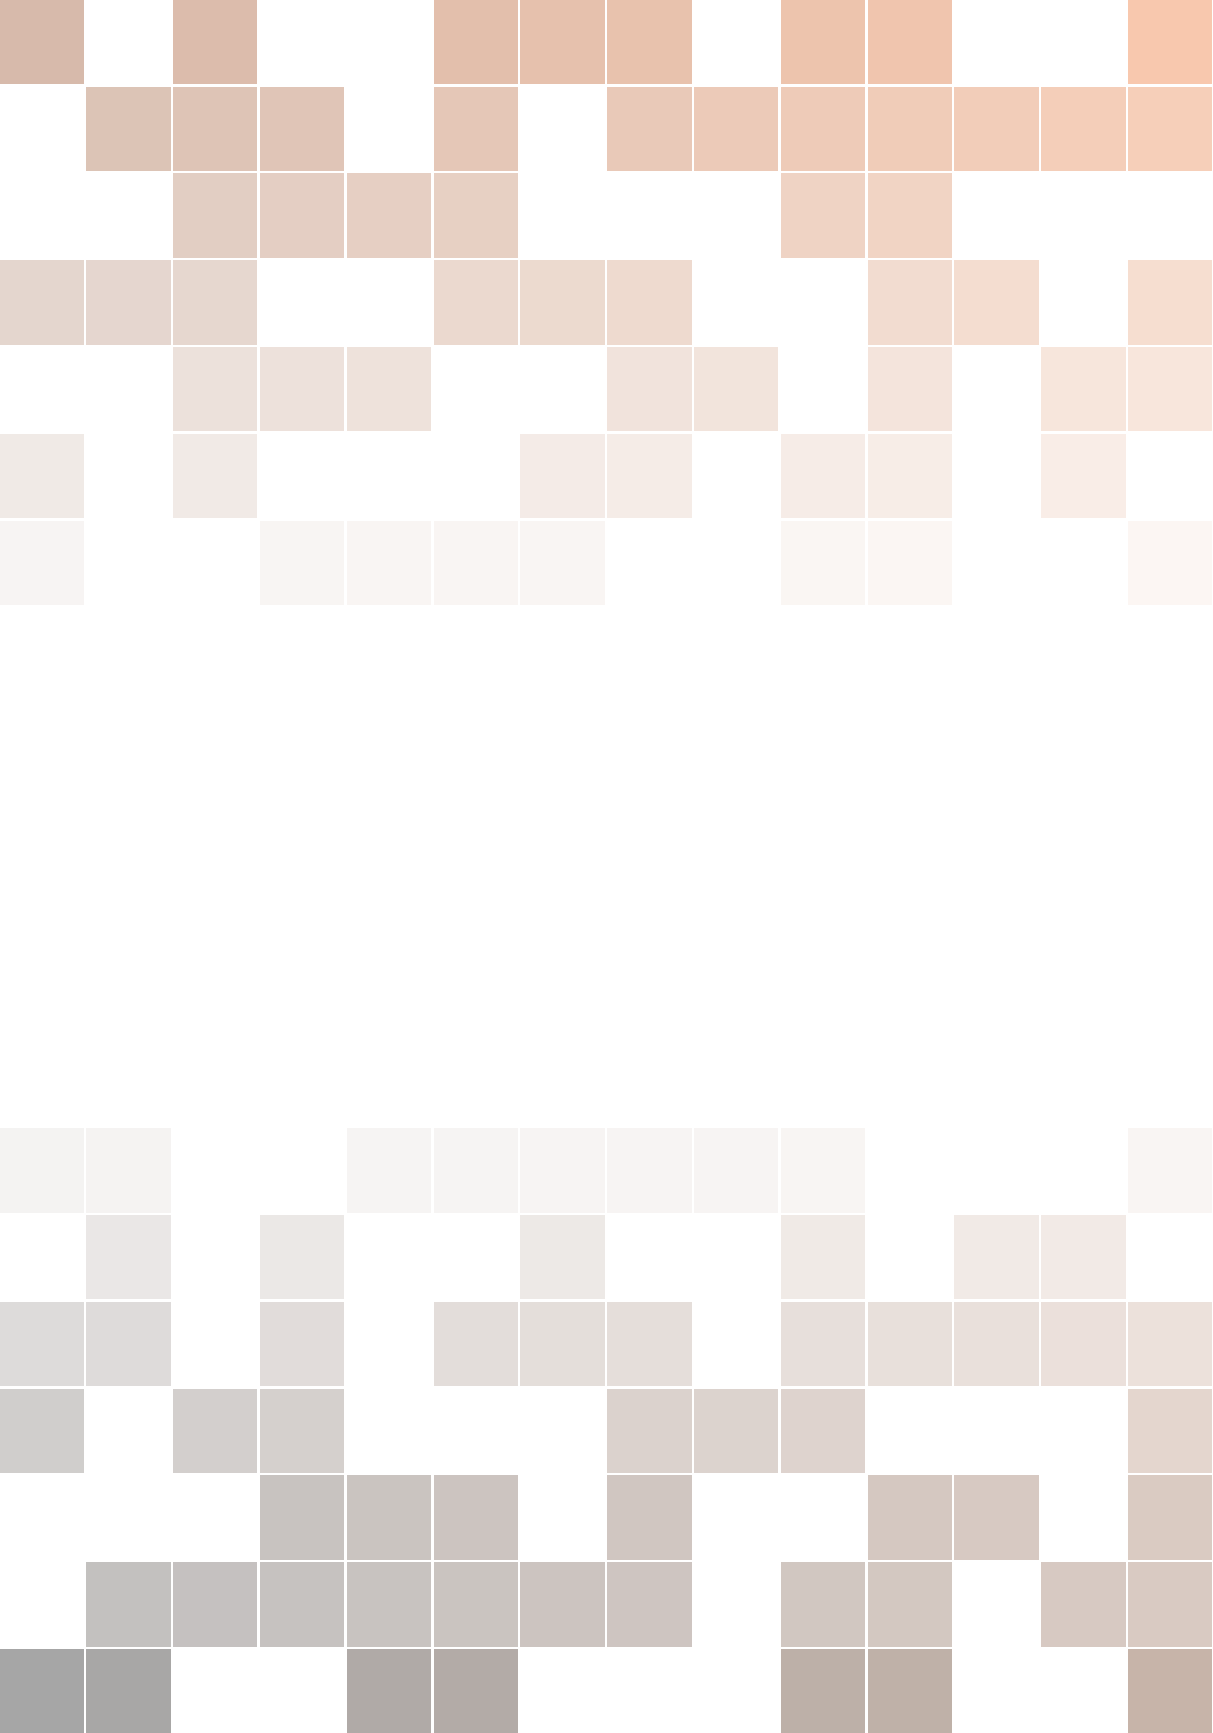
\includegraphics[width=\paperwidth]{background.pdf}};
\draw (current page.center) node [fill=ocre!30!white,fill opacity=0.6,text opacity=1,inner sep=1cm]{\Huge\centering\bfseries\sffamily\parbox[c][][t]{\paperwidth}{\centering Computation and Information\\[15pt] % Book title
{\Large Before quantum computers}\\[20pt] % Subtitle
}}; % Author name
\end{tikzpicture}
\vfill
\endgroup

%----------------------------------------------------------------------------------------
%	COPYRIGHT PAGE
%----------------------------------------------------------------------------------------

\newpage
~\vfill
\thispagestyle{empty}

\noindent Copyright \copyright\ 2019 David Elkouss, Carmen Garc\'ia Almudever \& Ryoichi Ishihara\\ % Copyright notice

%\noindent \textsc{Published by Publisher}\\ % Publisher

%\noindent \textsc{book-website.com}\\ % URL

\noindent Licensed under the Creative Commons Attribution-NonCommercial 3.0 Unported License (the ``License''). You may not use this file except in compliance with the License. You may obtain a copy of the License at \url{http://creativecommons.org/licenses/by-nc/3.0}. Unless required by applicable law or agreed to in writing, software distributed under the License is distributed on an \textsc{``as is'' basis, without warranties or conditions of any kind}, either express or implied. See the License for the specific language governing permissions and limitations under the License.\\ % License information, replace this with your own license (if any)

%\noindent \textit{First version, March 2019} % Printing/edition date

%----------------------------------------------------------------------------------------
%	TABLE OF CONTENTS
%----------------------------------------------------------------------------------------

%\chapterimage{chapter_head_eniac.jpg} % Table of contents heading image

\pagestyle{empty} % Disable headers and footers for the following pages

\tableofcontents % Print the table of contents itself

\cleardoublepage % Forces the first chapter to start on an odd page so it's on the right side of the book

\pagestyle{fancy} % Enable headers and footers again

%\chapter*{Foreword}
\addcontentsline{toc}{chapter}{\textcolor{ocre}{Foreword}} % Add a Bibliography heading to the table of contents
We are in the middle of the so-called informatoin society. Most of our interactions are mediated in one or another way by communication and computation devices which also majoritarily are connected to the internet. This information society facilitates many of our tasks, from looking for a neearby supermarket to learning about the best treatment for whatever illness we have or think we have (don't). It guides our choice of job, our application for job positions and allows us to communicate with distant relatives and also with friends that might be a few meters away from us. All this wealth of possibilities capable of satisfying our pst needs and drivign force of needs we did ot have a few years ago, relies on mathematical tools and models that did not exist until very recently. In fact some of these tools were thought to be impossible until they wre proved wrong. Even while part of the information society, we are also in the middle of a revolution, that is taking us from the world of classical information to a new world were information follows the strange laws of quantum mechanics. We expect much of this new world, amazing speed ups in computation, that will allow to discover new drugs, produce unhackable communication systems or improve our observations of the distant universe. However, what does it mean to speed up, what are the limits of the classical world? In which sense are some problems untractable by the computers we know today? Sure, it is only a matter of buying enough computation power and then we could also achieve the feats mentioned before, or perhaps is there some catch? It turns out, that there are problems that no computation device can solve, problems that can be computed but are beyond the reach of quantum computers. In fact, most of the problems that classical computers can deal with, can also be dealt with by quantum computers with no speed up. It is only for a limited number, of highly structured problems that quantum ocmputers promise to offer amazing improvement. However, still for those problems the speed up is in terms of how the computation resources necessary grow with the size of the problem. What is even information?



\part{Computation}
%%----------------------------------------------------------------------------------------
%	CHAPTER 1
%----------------------------------------------------------------------------------------

\chapterimage{chapter_head_eniac.jpg} % Chapter heading image

\chapter{Computer architecture}

\booksection{The von Neumann architecture}

\lipsum[1-7] % Dummy text

%------------------------------------------------

\booksection{Layered architecture: from applications to physics}

This statement requires citation \cite{article_key}; this one is more specific \cite[162]{book_key}.

%------------------------------------------------

\booksection{Instruction set and instruction format}

\booksection{SIMD, MIMD}

\booksection{Single-core, homogeneous multi-core, heterogeneous multicore}

% Lists are useful to present information in a concise and/or ordered way\footnote{Footnote example...}.

% \subsection{Numbered List}

% \begin{enumerate}
% \item The first item
% \item The second item
% \item The third item
% \end{enumerate}

% \subsection{Bullet Points}

% \begin{itemize}
% \item The first item
% \item The second item
% \item The third item
% \end{itemize}

% \subsection{Descriptions and Definitions}

% \begin{description}
% \item[Name] Description
% \item[Word] Definition
% \item[Comment] Elaboration
% \end{description}
%%----------------------------------------------------------------------------------------
%	CHAPTER 2
%----------------------------------------------------------------------------------------

\chapterimage{chapter_head_eniac.jpg} % Chapter heading image

\chapter{Digital systems}

\booksection{Int}

\lipsum[1-7] % Dummy text

%------------------------------------------------

\booksection{Layered architecture: from applications to physics}

This statement requires citation \cite{article_key}; this one is more specific \cite[162]{book_key}.

%------------------------------------------------

\booksection{Instruction set and instruction format}

\booksection{SIMD, MIMD}

\booksection{Single-core, homogeneous multi-core, heterogeneous multicore}
%\chapterimage{chapter_head_eniac.jpg} % Chapter heading image

\chapter{Logical gates}

\booksection{Table}

\begin{table}[h]
\centering \begin{tabular}{l l l}
\toprule
\textbf{Treatments} & \textbf{Response 1} & \textbf{Response 2}\\
\midrule
Treatment 1 & 0.0003262 & 0.562 \\
Treatment 2 & 0.0015681 & 0.910 \\
Treatment 3 & 0.0009271 & 0.296 \\
\bottomrule
\end{tabular}
\caption{Table caption}
\label{tab:example} % Unique label used for referencing the table in-text %\addcontentsline{toc}{table}{Table \ref{tab:example}} % Uncomment to add the table to the table of contents
\end{table}

Referencing Table \ref{tab:example} in-text automatically.

%
\chapterimage{chapter_head_eniac.jpg} % Chapter heading image

\chapter{Finite state machines}
%------------------------------------------------

\booksection{Figure}
\begin{figure}[h]
\centering
\includegraphics[scale=0.5]{placeholder.jpg}
\caption{Figure caption}
\label{fig:placeholder} % Unique label used for referencing the figure in-text
%\addcontentsline{toc}{figure}{Figure \ref{fig:placeholder}} % Uncomment to add the figure to the table of contents
\end{figure}

Referencing Figure \ref{fig:placeholder} in-text automatically.

%\chapterimage{chapter_head_eniac.jpg} % Chapter heading image

\chapter{Computability}
%------------------------------------------------
\booksection{Algorithms}
\booksection{Turing machines}
\subsection{Construction}
\begin{example}
A Turing machine for adding a number.
\end{example}
\begin{example}
A Turing machine for recognizing strings in the set 
\end{example}
\subsection{Simulating more complicated machines}
\begin{itemize}
\item Binary encoding
\item Rational numbers
\end{itemize}
\booksection{Universal Turing machines}
\subsection{The number of a Turing machine}
\subsection{The universal machine}
\booksection{Undecidability}
\subsection{Decision problems}
\subsection{Halting problem}
\subsection{Undecidability of the halting problem}
\booksection{Further reading}

%\chapterimage{chapter_head_eniac.jpg} % Chapter heading image

\chapter{Complexity theory}
%------------------------------------------------

\booksection{From computability to complexity} 
\begin{remark}
All computable problems are computable,
but some of them are more computable than the rest.
\end{remark}
\booksection{Counting resources}
We can count time

We can count space

Time(n) is included in Space(n)
\booksection{Bachmann–Landau notation}
\begin{definition}
Big O
\end{definition}
\begin{definition}
Small O
\end{definition}
\begin{exercise}
Show that..
\end{exercise}
\begin{exercise}
Show that..
\end{exercise}
\booksection{The complexity zoo}
\subsection{P}
\begin{definition}
Class P
\end{definition}
\begin{example}
The problem...
\end{example}
\subsection{PSPACE}
\begin{definition}
Class PSPACE
\end{definition}
\begin{example}
The problem...
\end{example}
\subsection{EXP}
\begin{definition}
Class EXP
\end{definition}
\begin{example}
The problem...
\end{example}
\subsection{NP}
\begin{definition}
Class NP
\end{definition}
\begin{example}
The problem...
\end{example}
\subsection{Probabilistic computation}
\begin{definition}
Class NP
\end{definition}
\begin{example}
The problem..
\end{example}
\booksection{From decision problems to arbitrary problems}
\booksection{Further reading}


\part{Information}
\usechapterimagetrue
\chapterimage{chapter_head_shannon.jpg} % Chapter heading image
\chapter{Measures of information}
\usechapterimagefalse
%------------------------------------------------
This is the age of information.
We open documents, consume media, exchange text messages, perform videoconferences or watch the weather forecast to name a few examples.
But what is exactly information? Can we quantify it? Is it possible to say that
one weather forecast contains more information than another? In this chapter,
we will learn that this is indeed possible. Our exposition, follows to a great
extent the visionary paper of Claude Shannon in 1948.

\booksection{Surprising information}
Let us warm up with a series of questions. 
The premise of all of them is the following: 
For some reason you want to know the weather forecast for tomorrow, but don't want to watch it or read it yourself. 
However, in order to get some information that allows you to choose appropriately your clothing for the next day, you ask a friend to send you a message to your phone every night with a summary of the forecast. 
You agree on a very simple encoding for the message, your friend will send a $1$ if the forecast predicts precipitations and $0$ otherwise. Think about these questions and come back to them after reading the whole chapter.
\begin{table}[h!]
  \begin{center}
    \label{tab:table1}
    \begin{tabular}{l|l|l} 
      \textbf{Location} & \textbf{Days of rain} & \textbf{Days with no rain}\\
      \hline
      \text{Rotterdam\footnote{source:knmi.nl}} & 153 & 212\\%\footnote{source:knmi.nl}
      \text{Atacama desert} & 5 & 360
    \end{tabular}
    \caption{Summary of precipitations in the year 2018.}
  \end{center}
\end{table}
\begin{exercise}
Let us assume that you are living in the Atacama desert where it rarely rains and you receive a $0$. How much information does this message carry? 
\end{exercise}
\begin{exercise}
Now let us assume that you live in the Netherlands where it does rain quite often, but certainly not every day. You also receive a $0$, does the message contain information? What about if you receive a $1$? Does the $1$ message contain more or less information than the message $0$? 
\end{exercise}
\begin{exercise}
\label{ex:infcontext}
Finally, let us assume that you live in the Netherlands and you happen to know that it is mid August. Does the message $0$ carry the same information as in winter?
\end{exercise}

Before you continue reading, pause for a moment and think what is common in your answers.

We have posed these questions to suggest a relation between the amount of information a message provides and how surprising it is. 
We will make this connection stronger in the rest of these chapter. %Now, what other properties do you think an information measure should satisfy?
%Information is never negative, i.e. if we know already the content of a message, we can say that it contains zero information. 
%This is the worst case, in any other case, the content of the message will always complement our understanding of the world and will in consequence contain some information. 
%Finally, the information we learn, when we learn about unrelated events should add up. 
%The sum of the informatio nthat we elarn when we know that tomorrow will rain and the one we learn when we know that we have won the lottery should be the same as the information we learn when we learn both events. However, as we saw in the weather information, context does play a role. Learning that it will rain, will have different value depending on the location or on the time of the year. In the following we will make use of our desided properties of an information quantity and find a mathematical function that fulfills them all.

\booksection{Refresher on probability theory}
A basic understanding of probability theory is essential for the material that follows. 
Let us review the fundamental concepts and definitions together with the notation that we will use here. 
As we will only deal with discrete probability distributions, the definitions that follow are not fully general but sufficient for our purposes.
If you have troubles following this section and doing the exercises please go back to your undergraduate text on the topic. 

Given a finite set $\mathcal X$, we call a probability distribution a function $p:\mathcal X\rightarrow[0,1]$, that is a function from the elements of $\mathcal X$ to the closed interval in the real line between zero and one, with the condition that $\sum_{x\in\mathcal X}p(x)=1$. 
Note that it follows automatically from our definition that for all $x\in\mathcal X$ $p(x)\geq 0$. 
\begin{example} Let $\mathcal X =\left\{\text{tails},\text{heads}\right\}$ we could define a probability distribution function $p$ such that $p(\text{heads})=0.3$ and $p(\text{tails})=0.7$.
\end{example}
\begin{example} An important example is the uniform distribution. Given a finite set $\mathcal X$, a uniform distribution on the set $\mathcal X$ is a function $p$ that for all $x\in\mathcal X$ assigns the value $$p(x)=\frac{1}{|\mathcal{X}|}\ .$$ where, we denote by $|\cdot|$ the number of elements in the set.
\end{example}
We define an ensemble $X$ as the tuple of a probability distribution $p_X$ together with its domain $\mathcal A_X$. 
Generally, we will refer to $\mathcal A_X$ as the sample space of $X$ and to its elements as events. %and its elements differently depending on the context. as the sample space and to any non empty subset of it as an event. 
In information theory, $X$ typically models an object in a communications setup (see \ref{}), in this context it is common to call $\mathcal A_X$ the alphabet of $X$ and refer to its elements as letters. %and its elements differently depending on the context. as the sample space and to any non empty subset of it as an event. 

Note that we can extend the definition of $p_X$ to any subset $\mathcal{S}\subseteq \mathcal{A}_X$:
\begin{equation}
p_X(\mathcal{S})=\sum_{x\in \mathcal{S}}p_X(x)
\end{equation} 
\begin{example}
Let $X$ be an ensemble with alphabet $\mathcal A_X=\{1,2,3\}$ and with $p_X$ the uniform distribution. Then if $\mathcal S=\{1,2\}$, $p(\mathcal S)=1/3+1/3=2/3$ 
\end{example}
Abusing notation, we will also call event any subset of the alphabet of an ensemble. For this particular case of set we will drop the caligraphic notation for sets.
Let $a$ and $b$ be two events in $\mathcal{X}$, we define $a\cup b$ and $a\cap b$ as the union and intersection of $a$ and $b$. 
$a\cup b$ is the event that contains all outcomes belonging to $a$, to $b$ and to both, we will also denote the event $a\cup b$ by $a \text{ or } b$. 
$a\cap b$ is the event that contains all outcomes belonging to both $a$ and $b$, we will also denote the event $a\cap b$ by $a \text{ and } b$. Two events are disjoint if their intersection is null.

Given an ensemble $X$ and two events $a,b$ we say that they are independent if:
\begin{equation}
p_X(a \text{ and } b)=p_X(a)p_X(b)
\end{equation}
Let $a$ and $b$ be two events with non zero probability. We call $p_X(a|b)=p_X(a \text{ and } b)/p_X(b)$ the conditional probability of $a$ given that $b$ occurs. It follows that if and only if $a$ and $b$ are independent $p_X(a|b)=p_X(a)$.

In the following, we will use the explicit notation $p_X,\mathcal A_X$ for the probability distribution of ensemble $X$ and its alphabet whenever confusion can arise but we will drop the subscript whenever possible.
\begin{exercise}
Let $X$ be an ensemble modelling two fair coins. Identify two events $a,b$ that are independent and verify that $p_X(a|b)=p_X(a)$
\end{exercise}
\begin{solution}
A
\end{solution}
Given two alphabets $\mathcal A_X,\mathcal A_Y$ we can define a joint ensemble on them with sample space or alphabet the direct product: $\mathcal A_{XY} = \mathcal A_X \times \mathcal A_Y$. 
We can associate, as well, a probability distribution function to map all tuples $(x,y)$ to $[0,1]$. 

The probability of an event in the joint ensemble is equally defined as the sum of the probability of the individual events. 
In particular, we can define for every $x\in\mathcal X$ the probability of $p_X(x)$ as the sum of $p_{XY}(x,y)$ for all $y\in\mathcal Y$:
\begin{equation}
p_X(x)=\sum_{y}p_{XY}(x,y)
\end{equation} 
\noindent and equivalently $p_Y(y)$:
\begin{equation}
p_Y(y)=\sum_{x}p_{XY}(x,y)
\end{equation} 
\begin{example}
Consider $n$ repetitions of an experiment, each repetition can be modelled by ensemble $X$ and events in different experiments are independent. We can model the set of $n$ repetitions via the joint ensemble $X_1\ldots X_N$, where $X_i$ is the ensemble associated with the $i$-th experiment, and joint the probability distribution is given by:
\begin{equation}
p_{X_1\ldots X_N}(x_1,x_2,\ldots,x_n)=\prod_{i=1}^np_X(x_i)
\end{equation}
\end{example}
A random variable $V$ on the ensemble $X$ is a numerical function from the elements of $\mathcal A_X$ to (typically) the real line. That is, a function $V:\mathcal{A}_X\rightarrow \mathcal A_V$, where $\mathcal A_V$ is a finite subset of the reals. The random variable $V$ induces an ensemble with alphabet $\mathcal A_V$ and probability distribution $p_V$ where $p_V$ is given by:

\begin{equation}
p_V(v)=\sum_{x\in\mathcal A_X:V(x)=v}p_X(x)
\end{equation} 
for all $v\in\mathcal A_V$.

The mean or expectation of a random variable is given by:
\begin{equation}
\mathbb E[V]=\sum_{x\in\mathcal A_X}p_X(x)V(x)=\sum_{v\in\mathcal A_V}p_Vv
\end{equation}

\booksection{Axiomatic derivation of entropy}
\label{sec:axent}
Let us now try to understand what type of functions can quantify information in a satisfactory way. Let us make this investigation more precise. In particular, suppose that given some ensemble $X$ we observe the occurrence of an event $x\in\mathcal A_X$. As we informally argued in the introduction, the information we gain seems to be related to the likelihood of the event we observed. But how can we make this intuition quantitative? %What information does the observation provide?

A function that quantifies information will be a function from a subset of $\mathcal A_X$ to the reals. 
Let us call this function $h$. 
Then given some event $x$, $h(x)$ will be some number that will quantify the information we learn. 
Let us discuss what properties an ideal information quantifier should have. 

\begin{itemize}
\item The measure should be non-negative, that is, an event gives either none or some information, but it can not give negative information. That is, for all events $x\in\mathcal A_X$ we require:
         \begin{equation}
         h(x)\geq 0         
         \end{equation}
\item Suppose that we buy two lottery tickets in two different lottery games, event $x$ is: "our first ticket wins a prize", event $y$ is: "our second ticket does not win a prize". 
We expect these two events to be independent and the information content of knowing both events should be the sum of the information of the individual events.
The occurrence of two independent events should yield the same information that the occurrence of the single events would provide an observer. If we let $h$ be an information measuring function
         \begin{equation}
         p_X(x \text{ and } y)=p_X(x) p_X(y)\Rightarrow h(x\text{ and } y) = h(x)+h(y)
         \end{equation}
         %and more generally the information that $n$ independent identical events provide:
         %\begin{equation}
         %\label{eq:indepentr}
         %h(a^n) = nh(a)         
         %\end{equation}
\item Following our discussion about information and surprise, we want $h$ to quantify less probable events with a larger value than more probable events. For any two ensembles $X,Y$ and events $x\in\mathcal A_X$ and $y\in\mathcal A_Y$, we require:
         \begin{equation}
         \label{eq:incentr}
         p_X(x)< p_Y(y) \Rightarrow h(x)> h(y)
         \end{equation}
\item The final condition is that we don't want that arbitrarily small changes in probability lead to a change in the information quantity, i.e. $h$ should be a continuous function.     
\end{itemize}

It turns out that there is a very limited set of functions that verify these properties. Given some ensemble $X$, the unique family of functions is of the form: 
\begin{equation}
\label{eq:h}
         h(x) = -\log_\lambda p_X(x)
\end{equation}
\noindent where $x\in\mathcal A_X$ and with $\lambda > 1$ for the measure to be positive. 
Choosing different values of $\lambda$ allows us to measure information with different units. 

There are some common choices of $\lambda$ that give rise to well known units of information: if we let $\lambda=2$, the unit of information is called bit. When $\lambda=3$ information is measured in trits, for $\lambda=10$ the unit is called a digit and when $\lambda=e$ nat. Unless stated otherwise, in the following we will assume that $\lambda=2$ and will let $\log=\log_2$.
\begin{definition}
Given an ensemble $X$ the information measured in bits of an event $S\subset \mathcal A_X$ is given by:
\begin{equation}
h(\mathcal S) = -\log p_X(\mathcal S)
\end{equation}
\end{definition}
\begin{exercise}
Let $X$ be an ensemble modelling a fair coin, that is with alphabet $\mathcal A_X=\{\text{heads},\text{tails}\}$ and with $p_X$ the uniform distribution. What is the information of the event heads and of the event tails?
\end{exercise}
\begin{solution}
As $p_X$ is uniform, we have that $p(\text{heads})=p(\text{tails})=1/2$. Hence:
\begin{equation*}
h(\text{heads})=-\log(1/2)=1\text{ bit}
\end{equation*}
and
\begin{equation*}
h(\text{heads})=-\log(1/2)=1\text{ bit}\ .
\end{equation*}
\end{solution}
Let us end this section by checking that all our desired conditions hold. First since the $\log$ function is continuous and monotonically increasing in the range $(0,1]$ it holds that $h$ is also continuous and monotonically decreasing in the range. Finally, if two events $a,b$ are independent, $p(a \text{ and } b)=p(a)p(b)$ and in consequence 
\begin{align}
h(a \text{ and } b) &= -\log \left(p(a \text{ and } b)\right)\\
                    &= -\log \left(p(a) p(b)\right)\\
                    &= -\log(p(a)) -\log(p(b))\\
                    &= h(a)+h(b)
\end{align}
\booksection{Entropy}
\label{subsec:entropy}
We define the entropy of an ensemble as the average information content it provides:
\begin{definition} Let $X$ be an ensemble, the entropy of the ensemble is defined as: 
        \begin{equation}\label{eq:entr}
        H(\mathbf{X})=-\sum_{x} p(x)\log p(x)   
        \end{equation}
\noindent where we take the convention that $0\log 0=0$, i.e. adding a  zero-probability event to a source does not affect its entropy.
\end{definition}
We can rewrite the definition of entropy as the expectation of the random variable $h(X)$. That is a random variable that associated each event with the negative logarithm of its probability: 

\begin{equation}
  \label{eq:mean}
  H(\mathbf{X})=-\sum_{x} p(x)\log p(x) = E(-\log p(\mathbf{X}))
\end{equation}

Note that entropy only depends on the values of the probabilities. In the following we will sometimes be interested in the entropy a probability distribution independently of an ensemble. We will use the notation $H(p_1,\ldots,p_n)$ to indicate the probability distribution. Let us now investigate some basic properties of entropy that we will use through this course.

\begin{exercise}Show that entropy can not be negative.
  \label{lem:entropynonnegative}
  \begin{equation*}
    H(\mathbf{X})\geq 0
  \end{equation*}
\end{exercise}
\begin{solution}
  \begin{equation}
    0 \leq p(x) \leq 1 \Rightarrow -\log p(x) \geq 0 \Rightarrow H(X) \geq 0
  \end{equation}
\end{solution}

%\begin{definition} A function $f(x)$ defined on the interval $(a,b)$ is concave if any two points $x_1$, $x_2$ in the interval and any $t\in[0,1]$ verify:
%        \begin{equation}
%        f(tx_1+(1-t)x_2) \geq tf(x_1)+(1-t)f(x_2)
%         \end{equation}
%\end{definition}

%We prove the corollary of Jensen's inequality for concave functions as it demonstrates the non-negativity of the entropy function~\cite{Cover_91}.

The following is known as Jensen's inequality and will be of use in the following. See~\cite{Cover_91} for a proof.
\begin{theorem}[Jensen's inequality] Let $f$ be a concave function and $X$ a random variable. Then: 
  \label{th:jensen}
  \begin{equation*}
    f(E(\mathbf{X}))\geq E(f(\mathbf{X}))
  \end{equation*}
\end{theorem}
%
%\begin{proof}
%  We proceed to show by induction on the number of elements  in $\mathcal{X}$.
%  \begin{equation}
%    \label{eq:jensenbasis}
%    f(p_1x_1+p_2x_2) \geq p_1f(x_1)+p_2f(x_2)
%  \end{equation}
%  \noindent Eq.~\ref{eq:jensenbasis}, that follows from the concavity of $f(x)$, shows that Jensen's inequality holds for $|\mathcal{X}|=2$, if we assume that it holds for $|\mathcal{X}|=n$:
%
%  \begin{equation}
%    f(\sum_{i=1}^np_ix_i) \geq \sum_{i=1}^np_if(x_i)
%  \end{equation}
%  \noindent the induction hypothesis implies that it should also hold for $|\mathcal{X}|=n+1$
%
%  \begin{eqnarray}
%    f(\sum_{i=1}^{n+1}p_ix_i) 
%        & =    & f\left( p_{n+1}x_{n+1} + (1-p_{n+1}) \sum_{i=1}^{n}\frac{p_i}{1-p_{n+1}}x_i \right) \nonumber \\
%        &\geq & p_{n+1}f(x_{n+1}) + (1-p_{n+1}) f\left( \sum_{i=1}^{n}\frac{p_i}{1-p_{n+1}}x_i \right) \nonumber \\
%        &\geq & p_{n+1}f(x_{n+1}) + (1-p_{n+1}) \sum_{i=1}^{n}\frac{p_i}{1-p_{n+1}}f(x_i) \nonumber \\
%        & = &    p_{n+1}f(x_{n+1}) + \sum_{i=1}^{n}p_if(x_i) \nonumber \\
%        & = &   \sum_{i=1}^{n+1}p_if(x_i)
%  \end{eqnarray}
%  \noindent where the first inequality follows from the concavity of $f(x)$ and the second from the induction hypothesis.
%\end{proof}
%
%\begin{lemma}The entropy of the uniform distribution equals the logarithm of the number of elements.
%  \begin{equation*}
%    H(\dfrac{1}{n}, ..., \dfrac{1}{n}) = \log n
%  \end{equation*}
%\end{lemma}
%\begin{proof}
%  \begin{equation}
%    H(\dfrac{1}{n}, ..., \dfrac{1}{n}) = -\sum_{i=1}^n \dfrac{1}{n} \log \dfrac{1}{n} = \log n        
%  \end{equation}
%\end{proof}

\begin{lemma}
\label{lem:uniform}
The distribution that maximizes entropy for any alphabet is the uniform distribution.
\begin{equation*}
H(p_1, ..., p_n)\leq \log n
\end{equation*}
\end{lemma}
\begin{proof}
\begin{eqnarray}
H(p_1, ..., p_n)  - \log n & =      & \sum_{i=1}^n p_i \log \dfrac{1}{p_i} - \sum_{i=1}^n \dfrac{1}{n} \log n \nonumber \\
                                       & =      & \sum_{i=1}^n p_i \log \dfrac{1}{p_i} - \log n \sum_{i=1}^n \dfrac{1}{n} \nonumber \\
                                       & =      & \sum_{i=1}^n p_i \log \dfrac{1}{p_i} - \log n \sum_{i=1}^n p_i \nonumber \\
                                       & =      & \sum_{i=1}^n p_i \log \dfrac{1}{p_i} - \sum_{i=1}^n p_i \log n \nonumber \\
                                       & =      & \sum_{i=1}^n p_i \log \dfrac{1}{np_i} \nonumber \\                                      
                                       & \leq &  \log \sum_{i=1}^n \dfrac{1}{n} = 0\nonumber \\
\end{eqnarray}
\noindent where the second equality follows from the fact that a probability distribution adds up to one and the last inequality holds from $\log$ being a concave function and applying Jensen's inequality.
\end{proof}

%\subsection{Data Compression}
%Once presented an information measure, we review some of its operational interpretations, in particular its relation with the theoretical limits for data compression.
%
%A source code $C$ in alphabet $\mathcal{Y}$ for a random variable taking values in $\mathcal{X}$ is a function $c:\mathcal{X}\longrightarrow \mathcal{Y}^*$, where $\mathcal{Y}^*$ is any finite direct product of $\mathcal{Y}$. We call $c(x)$ the codeword for $x$ and $l(x)=|c(x)|$ the length of the codeword for $x$.
%
%The length of a source code $C$ is the sum of the lengths of every codeword in $C$ weighted by its relative frequency.
%\begin{equation}
%L(C(\mathbf X)) = \sum_{x} p(x) l(x)
%\end{equation}
%
%A source code is uniquely decodable if any concatenation of codewords can only be generated by a unique concatenation of source symbols. In other words, the source symbols generating the codewords can be recovered with no possible equivocation. 
%
%The next inequality on the length of uniquely decodable source codes was first proved by McMillan~\cite{McMillan_56} however the following proof is a simpler version by Karush~\cite{Karush_61,Cover_91}.
%
%\begin{theorem} The length of a uniquely decodable source code $C$ for a random variable $\mathbf{X}$ taking values in alphabet $\mathcal{Y}$ verifies:
%\begin{equation*}
%\sum_{x}\frac{1}{|\mathcal{Y}|^{l(x)}} \leq 1
%\end{equation*}
%\label{th:mcmillan}
%\end{theorem}
%\begin{proof}
%Let $c(x_1, x_2, ..., x_k)$ be a concatenation of codewords of aggregated length $l(x_1, x_2, ..., x_k)=\sum_{i=1}^k l(x_i)$. Since $C$ is uniquely decodable for any aggregated length $k$, no more than $|\mathcal{Y}|^k$ different concatenation of codewords can be generated. 
%
%We can consider the related expression on the aggregated length:
%\begin{eqnarray}
%\left( \sum_{x}\frac{1}{|\mathcal{Y}|^{l(x)}} \right)^n &=& \sum_{x_1}\frac{1}{|\mathcal{Y}|^{l(x_1)}} \sum_{x_2}\frac{1}{|\mathcal{Y}|^{l(x_2)}} \dots \sum_{x_n }\frac{1}{|\mathcal{Y}|^{l(x_n)}} \nonumber \\
%&=& \sum_{x_1,x_2,\dots,x_n }\frac{1}{|\mathcal{Y}|^{l(x_1)+l(x_2)+\dots +l(x_n)}} \nonumber \\
%&=& \sum_{x_1,x_2,\dots,x_n }\frac{1}{|\mathcal{Y}|^{l(x_1+x_2+\dots +x_n)}}
%\end{eqnarray}
%\noindent which can also be written as the sum for all possible lengths $i$ of the number $T_i$ of concatenation of $n$ codewords:
%
%\begin{eqnarray}
%\left( \sum_{x }\frac{1}{|\mathcal{Y}|^{l(x)}} \right)^n &=& \sum_{i=1}^{nl_{max}}\frac{T_i}{|\mathcal{Y}|^i} \nonumber \\
%&\leq & \sum_{i=1}^{nl_{max}}\frac{|\mathcal{Y}|^i}{|\mathcal{Y}|^i} \nonumber \\
%&\leq & nl_{max}
%\end{eqnarray}
%\noindent where $l_{max} = \max_{x}l(x)$. And taking the $n$-th root in both sides:
%
%\begin{eqnarray}
%\sum_{x }\frac{1}{|\mathcal{Y}|^{l(x)}}  &\leq & (nl_{max})^{1/n}
%\end{eqnarray}
%\noindent now since the limit $\lim_{n \to \infty } (nl_{max})^{1/n} = 1$ and the result holds for all $n$:
%
%\begin{eqnarray}
%\sum_{x }\frac{1}{|\mathcal{Y}|^{l(x)}}  &\leq 1
%\end{eqnarray}
%\end{proof}
%
%We finish this brief overview of source coding with Th.~\ref{th:sourcecoding}~\cite{Cover_91}, it shows that the length  of a uniquely decodable code is lower bounded by the entropy of the random variable.
%\begin{theorem}
%\label{th:sourcecoding}
%The length of a uniquely decodable code taking values from finite alphabet $\mathcal{Y}$ for random variable $\mathbf{X}$ is lower bounded by the entropy of $\mathbf{X}$.
%\begin{equation*}
%L\geq H_{|\mathcal{Y}|}(\mathbf{X})
%\end{equation*}
%\begin{proof}
%\begin{eqnarray}
%H_{|\mathcal{Y}|}(\mathbf{X}) - L &=& \sum_{x} p(x) \log_{|\mathcal{Y}|} \frac{1}{p(x)} - \sum_{x}p(x)l(x) \nonumber \\
%                                      &=& \sum_{x} p(x) \log_{|\mathcal{Y}|} \frac{1}{p(x)} - \sum_{x} p(x)  \log_{|\mathcal{Y}|} |\mathcal{Y}|^{-l(x)} \nonumber \\
%                                      &=& \sum_{x} p(x) \log_{|\mathcal{Y}|} \frac{|\mathcal{Y}|^{-l(x)} }{p(x)} \nonumber \\
%                                      &\leq & \log_{|\mathcal{Y}|} \sum_{x} |\mathcal{Y}|^{-l(x)} \nonumber \\
%                                      &\leq & \log_{|\mathcal{Y}|} 1 = 0
%\end{eqnarray}
%\noindent where the first inequality is again an application of Jensen's result Th.~\ref{th:jensen} and the second one results from applying McMillan's Th.~\ref{th:mcmillan}.
%\end{proof}
%\end{theorem}
%
%This result can be extended to consider a source code $C$ for a sequence of $n$ random variables {iid} from the ensemble $\mathbf{X}$. That is, a source  $\mathbf{X}$ as we defined it in Sec.~\ref{subsec:entropy}. Let $R=L(C(\mathbf {X^n}))/n$, the length per symbol of $C$, be the encoding rate of the source $\mathbf{X}$. It is trivial to see that the rate is also lower bounded by the entropy of the source:
%
%\begin{eqnarray}
%R &=& L(C(\mathbf {X^n}))/n \nonumber\\
%  &\geq& H_{|\mathcal{Y}|}(\mathbf{X^n})/n \nonumber\\
% &=& H_{|\mathcal{Y}|}(\mathbf{X})
%\end{eqnarray}

\booksection{Joint entropy, conditional entropy and mutual information}
We will now explore three information measures that derive from entropy as we defined it in the previous section. The first measure is joint entropy, which is a direct application of the definition of entropy to a joint source.
\begin{definition}
Given two ensembles $\mathbf{X}$ and $\mathbf{Y}$ the entropy of the joint ensemble $XY$ is given by:
\begin{equation}
H(\mathbf{XY}) = - \sum_{x,y} p(x,y)\log p(x,y)
\end{equation}
\end{definition}

Exercise \ref{ex:infcontext} suggests that the information content depends on the context. The second information measure that we introduce is conditional entropy.
First, we can extend in a straightforward way the reasoning in Sec.~\ref{subsec:information} to define an information measure conditional on the knowledge of some event $y$. 
It can analogously be proved that a conditional information measure is of the form: 
\begin{equation}
h(a|b) = -\log p (a|b)
\end{equation}
Let $XY$ be a joint ensemble, we can define the conditional entropy of $X$ given the event $y$ as the average conditional information:
\begin{equation}
H(\mathbf{X}|y) = \sum_x p(x|y) h(x|y)
\end{equation}
and the conditional entropy of $X$ given ensemble $Y$:
\begin{equation}
H(\mathbf{X}|\mathbf{Y})=\sum_yH(X|y)
\end{equation}
\begin{exercise}
Show that $H(X|Y)=H(XY)-H(Y)$.
\end{exercise}
Let us investigate some basic properties of the conditional entropy.
\begin{exercise}Show that the conditional entropy is non-negative.
\begin{equation*}
H(\mathbf{X}|\mathbf{Y}) \geq 0
\end{equation*}
\end{exercise}
\begin{solution}
$H(\mathbf{X}|\mathbf{Y})$ is a sum of entropies, which are positive by Lem.~\ref{lem:entropynonnegative}, weighed by the probabilities of each event which are also positive.
\end{solution}

\begin{exercise}
\label{lem:entgeqcond}
Show that the entropy of the random variable $\mathbf{X}$ given any random variable $\mathbf{Y}$ is not greater than the entropy of $\mathbf{X}$.
\begin{equation*}
H(\mathbf{X}|\mathbf{Y}) \leq H(\mathbf{X})
\end{equation*}
\end{exercise}
\begin{solution}
\begin{eqnarray}
H(\mathbf{X}|\mathbf{Y}) - H(\mathbf{X}) &=& \sum_{y }p(y) \sum_{x} p(x|y)\log \frac{1}{p(x|y)} - \sum_{x}p(x) \log  \frac{1}{p(x)}\nonumber \\
                         &=& \sum_{y}\sum_{x}p(x,y) \log \frac{1}{p(x|y)} + \sum_{x,y}p(x,y) \log  p(x) \nonumber \\
                         &=& \sum_{x,y}p(x,y) \log  \frac{p(x)}{p(x|y)} \nonumber \\
                         &=& \sum_{x,y}p(x,y) \log  \frac{p(x)p(y)}{p(x,y)} \nonumber \\
                         &\leq & \log \sum_{x,y} p(x) p(y) = 0
\end{eqnarray}
\end{solution}

\begin{exercise}
\label{lem:function}
Given random variables $\mathbf{X}$ and $\mathbf{Y}$ if $\mathbf{X}=f(\mathbf{Y})$: 
\begin{equation*}
H(\mathbf{X}|\mathbf{Y}) = 0
\end{equation*}
\end{exercise}
\begin{solution}
If $\mathbf{X}=f(\mathbf{Y})$, then given $\mathbf{Y}$ we know $\mathbf{X}$ with absolute certainty, in other words, given $\mathbf{Y}$ there is just one possible outcome.
\begin{eqnarray}
H(\mathbf{X}|\mathbf{Y})&=&\sum_{y}p(y) H(\mathbf{X}|y)\nonumber\\
         &=& 0
\end{eqnarray}
\end{solution}

%We now derive the so called chain rule of joint entropy.

\begin{exercise} Show that the following relation holds for any two ensembles $XY$:
\begin{equation*}
H(\mathbf{XY}) = H(\mathbf{X}) + H(\mathbf{Y}|\mathbf{X})
\end{equation*}
\end{exercise}
\begin{solution}
\begin{eqnarray}
H(\mathbf{XY}) &=& - \sum_{x,y} p(x,y)\log p(x,y) \nonumber \\
       &=& - \sum_{x}p(x)\sum_{y} p(y|x)\log p(x)p(y|x) \nonumber \\
       &=& - \sum_{x}p(x)\log p(x)\sum_{y} p(y|x) \nonumber \\
       & & - \sum_{x}p(x)\sum_{y} p(y|x)\log p(y|x) \nonumber \\
       &=& H(\mathbf{X}) + H(\mathbf{Y}|\mathbf{X})
\end{eqnarray}
\end{solution}

%The joint and conditional entropy definitions can be also naturally extended to multiple variables. %We show a %second 
%chain rule for the joint entropy of $\mathbf{X}$ and $\mathbf{Y}$ given a variable $\mathbf{Z}$.  
%\begin{lemma}
%\label{lem:chain2}
%Let $\mathbf{X}$, $\mathbf{Y}$, and $\mathbf{Z}$ be three random variables, then:
%\begin{equation*}
%H(\mathbf{XY}|\mathbf{Z}) = H(\mathbf{X}|\mathbf{Z}) + H(\mathbf{Y}|\mathbf{X}\mathbf{Z})
%\end{equation*}
%\end{lemma}
%\begin{proof}
%\begin{eqnarray}
%H(\mathbf{XY}|\mathbf{Z}) &=& - \sum_{z}p(z)H(\mathbf{X}\mathbf{Y}|z)\nonumber \\
%         &=& - \sum_{z}p(z) \sum_{x,y} p(x,y|z)\log p(x,y|z) \nonumber \\
%         &=& - \sum_{z}p(z) \sum_{x} p(x|z)\sum_{y} p(y|xz)\log p(x|z)p(y|xz) \nonumber \\
%         &=& - \sum_{z}p(z) \sum_{x} p(x|z)\log p(x|z)\sum_{y} p(y|xz) \nonumber \\
%         & & - \sum_{z}p(z) \sum_{x}p(x|z)\sum_{y} p(y|xz)\log p(y|xz)  \nonumber \\ 
%         &=& H(\mathbf{X}|\mathbf{Z}) + H(\mathbf{Y}|\mathbf{X}\mathbf{Z})  
%\end{eqnarray}
%\end{proof}

The third information measure that we introduce is the mutual information:
\begin{definition}
Given a joint ensemble $XY$, we define the mutual information between $X$ and $Y$ by:
\begin{equation*}
I(X;Y)=H(X) + H(Y) - H(XY)
\end{equation*}
\end{definition}
The mutual information $I(\mathbf{X};\mathbf{Y})$ is a measure of the information shared between the two variables $\mathbf{X}$ and $\mathbf{Y}$. Let us make this intuition more precise:
\begin{exercise}
Show that for any ensemble $X$: $I(X;X)=H(X)$.
\end{exercise}
\begin{exercise}
Show that $I(X;Y)=0$ if and only if $X$ and $Y$ are independent. 
\end{exercise}
\begin{exercise}
Show that $I(X;Y)\geq 0$
\end{exercise}

Fig.~\ref{fig:infmeasures} shows the relationship between the four measures that we have defined: entropy, joint entropy, conditional entropy and mutual information.

\begin{figure}
\begin{center}
\def\svgwidth{.8\columnwidth} 
\input{figures/infmeasures.pdf_tex} 
\caption{Graphical representation of the information measures.}
\label{fig:infmeasures}
\end{center}
\end{figure}

\begin{eqnarray}
\label{eq:mutualinformation}
I(\mathbf{X};\mathbf{Y}) &=& H(\mathbf{Y}) - H(\mathbf{Y}|\mathbf{X}) \nonumber\\
         &=& H(\mathbf{X}) - H(\mathbf{X}|\mathbf{Y}) \nonumber\\
         &=& I(\mathbf{Y};\mathbf{X})
\end{eqnarray}
\booksection{Exercises}
\begin{exercise}
Let $X$ be a random variable with $H(X)>0$ and let $Y=f(X)$. 
\begin{enumerate}
\item Give one function such that $H(Y)=H(X)$
\item Give one function such that $0<H(Y)<H(X)$
\item Give one function such that $H(Y)=0$
\end{enumerate}
\end{exercise}
\begin{exercise}
A classic logical problem (also classic in information theory texts!) states that you receive 12 coins one of which is a counterfeit. The counterfeit is either lighter or heavier than the normal coins, you do not know which is the case. Fortunately, you have access to a two-plate scale that can compare weights.
\begin{enumerate}
\item Give a non-trivial bound on the minimum number of weighings that could give the answer.
\item Give an strategy that solves the problem if you know tha the counterfeit coin is heavier than normal coins.
\item Give an strategy that solves the general problem.
\end{enumerate}
\end{exercise}
\begin{exercise}
Convex mixtures
\end{exercise}
\begin{exercise}
Entropy of a sum goes to the minitest
\end{exercise}
\begin{exercise}
World series like exercise
\end{exercise}
\begin{exercise}
to minitet, for $X$, $Y$ independent $H(X,Y)=H(X)+H(Y)$.
\end{exercise}
\booksection{Further reading}
The mathematical foundations of information theory were to a certain extent developped single handedly by Claude Shannon. His original paper \cite{Shannon_48} developped the framework and also solved some of the most important problems. The text has not aged with time and remains a greatly written and accessible introduction to the field. A second excellent source for digging deeper into the material is the book of Cover and Thomas \cite{Cover_91}, it is the reference of the field and widely used in most introductory courses on information theory. 

In section \ref{sec:axent} we sketched an axiomatic derivation of entropy. For a complete discussion on axiomatic derivations of entropy and information please refer to~ \cite{Aczel_74,Aczel_75,Csiszar_08,Feinstein_58}. 

\usechapterimagetrue
\chapterimage{zip.png} 
\chapter{Data compression}
\usechapterimagefalse
%------------------------------------------------
In the previous chapter we posed a series of conditions that information measures should possess. We built on top of those conditions and found a series of information measures satisfying them. 

In this chapter we will begin a journey to show that not only entropy is a good measure for information according to our desired properties, but also that it carries a strong operational meaning. In fact, we will show that matching  our intuition, if an ensemble has a certain entropy, then the length of a message that can communicate the content of the ensemble can not be smaller the entropy of then ensemble. 

%We will also begin to investigate the difference between proofs of existence and constructive methods. This will be a common pattern in information theory, though of limited importance in our introductory course. In fact, it is in many circumstances, possible to prove that codes with desired properties must exist by relying on random ensembles of codes, while actually pointing an example is more complicated.

%something about zip files


\booksection{Codes}
\begin{definition}
A symbol code is a map $C:\mathcal A\mapsto\mathcal C^*$. We associate every symbol $a$ from the alphabet $\mathcal A$ with $C(a)$ a sequence of symbols from the code alphabet $\mathcal C$. We call $C(a)$ the codeword of $a$ and denote by $|C(a)|$ its length. %length notation elsewhere?
% define somewhere ^*
\end{definition}
\begin{example}
Let $X$ be an ensemble modelling a fair coin. We can consider the codes $C_1,C_2$ on the ensemble with: 

\noindent $C_1(\text{tails})=00$ and $C_1(\text{heads})=111$
\noindent $C_2(\text{tails})=0$ and $C_2(\text{heads})=0$
\noindent $C_3(\text{tails})=00$ and $C_2(\text{heads})=0$
\end{example}
%We could be more sophisticated. Let us assume that the four events occur with the following probability: it rains with probability $1/2$, it snows with probability $1/4$, and both sunny days and hailstone days happen with probability $1/8$. We could assign the following codewords to each event: rain $0$, snow $10$, sun $110$ and hail $111$. That is, we have assigned more likely events shorter codewords? Why is this better?
You have probably noticed that the code $C_2$ in the previous example is not very useful. This consideration motivates the following definitions.
\begin{definition}
A code $C:\mathcal X\mapsto\mathcal Y$ is non-singular if $\forall x,y\in\mathcal X$ with $x\neq y$ $C(x)\neq C(y)$.
\end{definition}
If we receive a single symbol encoded with a non-singular code, correct decoding is guaranteed, all codewords are different. However, we might consider the use of a code for sending a sequence of symbols from some ensemble. Let $X$ be an ensemble, $C$ be a code on the ensemble and $x=(x_1,\ldots,x_n)\in\mathcal X^*$ a sequence of elements of $\mathcal X$ with finite length. We can extend the definition of $C$ and define its action on $x$ as follows: $C(x)=C(x_1)C(x_2)\ldots C(x_n)$. That is, the word associated with $x$ is the concatenation of the codewords for $x_1$, $x_2$ until $x_n$. Under this extended definition, some non-singular codes can lead to erroneous decodings. For instance, consider the code $C_3$ in the previous example and the word $000$. It can be decoded both as (tails,heads) or as (heads,tails).
\begin{definition}
A code $C:\mathcal X\mapsto\mathcal Y$ is uniquely decodable if $\forall x,y\in\mathcal X^*$ with $x\neq y$ $C(x)\neq C(y)$.
\end{definition}
If we think in the usefulness of a code, unique decodability is a basic requirement. A more practical requirement is that it should be possible to decode symbols as one reads a word instead of waiting until the end of the transmission. 
A code is called instantaneous if it can be decoded symbol by symbol from left to right without regarding future symbols. 

A convenient family of instantaneous codes are so called prefix codes. Before defining them, let $w_1,w_2\in D^*$, $w_1$ is a prefix of $w_2$ if there exist $t\in D^*$ such that $w_1$ concatenated with $t$ equals $w_2$. That is: $w_1,t=w_2$.
\begin{definition}
A prefix code is a code where no codeword is the prefix of any other codeword.
\end{definition}
It is easy to see that prefix codes are instantaneous, indeed as soon as a complete codeword is seen, it is possible to decode the associated symbol. Since the codeword can not be prefix of a subsequent codeword, there is no possibility of confusion. Moreover, it turns out that all instantaneous codes are also prefix, i.e. both concepts are equivalent. In order to prove this, we can argue the contrapositive. 

Let $C$ be a non-prefix code and let's see that it implies it is not instantaneous. If $C$ is non prefix there exist codewords $w_1,w_2$ and $t$ such that $w_1,t=w_2$. Hence, if we receive $w_1$ we can not decode until additional symbols are received that allow to discriminate between $w_1$ and $w_2$.

\begin{exercise}
Let $w_1,w_2\in D^*$, $w_1$ is a suffix of $w_2$ if there exist $t\in D^*$ such that $t$ concatenated with $w_1$ equals $w_2$. We call a code a suffix code if no codeword is suffix of any other code word.
\begin{enumerate}
\item Are all suffix codes also prefix codes? If yes, prove it. If not, give a counterexample.
\item Are suffix codes uniquely decodable?
\item Are suffix codes instantaneous?
\end{enumerate}
\end{exercise}
In the previous example, it was fairly easy to spot that the code was not uniquely decodable. However, for some codes it is not so simple.
\begin{exercise}\label{ex:sardinas}
Let $C_1=\{01,100,1101,0111\}$ and $C_2=\{01,100,1101,10111,01011\}$. Are $C_1,C_2$ uniquely decodable? (Hint: if you can not find the solution, continue reading and return to this exercise once you have understood the Sardinas-Patterson method)
\end{exercise}

Let us now investigate a method to find if a code is uniquely decodable or not. This method was proposed by Sardinas and Patterson \cite{sardinas1953necessary} and is also known as the method of the dangling suffixes. 

The method works as follows:
\begin{enumerate}
\item Let $C_0$ be the set of codewords in the code
\item Let $C_1=\{w\in\mathcal A^*:uw=v,\text{ where }u,v\in C_0\}$.
\item For $n\geq 2$ do:
\begin{enumerate}
\item Let $C_n=\{w\in\mathcal A^*:uw=v,\text{ where }u\in C_0,v\in C_{n-1}\text{ or }u\in C_{n-1},v\in C_0\}$.
\item If $C_n$ is empty, the code is uniquely decodable
\item If there is $2\leq m<n$ such that $C_m=C_n$, i.e. if $C_n$ is a repeated set, then the code is uniquely decodable.
\item If the intersection between $C_0$ and $C_n$ is non-empty. That is if there is some codeword in $C_n$. Then the code is not uniquely decodable.
\item Else we increase $n$.
\end{enumerate}
\end{enumerate}

This method is a little bit magical. Let us informally investigate some of its properties. One might wonder about two things. First, does the algorithm end for all codes? This first question is relatively straight forward if one observes that the sets $C_n$ for $n\geq 2$ are always composed of suffixes of $C_0$. Since the number of possible suffixes is finite, the number of sets of suffixes is also finite. Hence at some point the algorithm will end. The second question is whether or not the output of the algorithm is correct. This is a little more complicated and beyond the scope of the course see \cite{Salomon2010} for more information.

\booksection{Code length and fundamental limits}
\begin{definition}
Given an ensemble $X$ and a code $C$ for this ensemble, we define the average length of the code as follows:
\begin{equation}
l(C)=\sum_{x\in\mathcal X}p(x)|C(x)|
\end{equation}
where $|C(x)|$ is the length of the codeword of event $x$.
\end{definition}
\begin{example}
Consider the codes $C_1,C_2$ for a fair coin. $C_1(\text{tails})=0$,  $C_1(\text{heads})=10$, $C_2(\text{tails})=0$, $C_2(\text{tails})=1$. The average length of the codes is:
\begin{align}
L(C_1)&=\frac{1}{2}1+\frac{1}{2}2=1.5\\
L(C_2)&=\frac{1}{2}1+\frac{1}{2}1=1
\end{align}
\end{example}
Intuitively, it seems that we can not do better than $C_2$, how do we prove it? In the following we prove a fundamental relation between the length of a code and the entropy of the associated ensemble. Previous to that we need to prove Kraft-MacMillan's inequality. This  inequality was first proved by McMillan~\cite{McMillan_56} however the following proof is a simpler version by Karush~\cite{Karush_61,Cover_91}.

\begin{theorem} \label{th:mcmillan}
The length of a uniquely decodable code $C$ for a random variable ${X}$ taking values in alphabet $\mathcal{Y}$ verifies:
\begin{equation*}
\sum_{x}\frac{1}{|\mathcal{Y}|^{l(x)}} \leq 1
\end{equation*}
\end{theorem}
\begin{proof}
Let $c(x_1, x_2, ..., x_k)$ be a concatenation of codewords of aggregated length $l(x_1, x_2, ..., x_k)=\sum_{i=1}^k l(x_i)$. Since $C$ is uniquely decodable for any aggregated length $k$, no more than $|\mathcal{Y}|^k$ different concatenation of codewords can be generated. 

We can consider the related expression on the aggregated length:
\begin{eqnarray}
\left( \sum_{x}\frac{1}{|\mathcal{Y}|^{l(x)}} \right)^n &=& \sum_{x_1}\frac{1}{|\mathcal{Y}|^{l(x_1)}} \sum_{x_2}\frac{1}{|\mathcal{Y}|^{l(x_2)}} \dots \sum_{x_n }\frac{1}{|\mathcal{Y}|^{l(x_n)}} \nonumber \\
&=& \sum_{x_1,x_2,\dots,x_n }\frac{1}{|\mathcal{Y}|^{l(x_1)+l(x_2)+\dots +l(x_n)}} \nonumber \\
&=& \sum_{x_1,x_2,\dots,x_n }\frac{1}{|\mathcal{Y}|^{l(x_1+x_2+\dots +x_n)}}
\end{eqnarray}
\noindent which can also be written as the sum for all possible lengths $i$ of the number $T_i$ of concatenation of $n$ codewords:

\begin{eqnarray}
\left( \sum_{x }\frac{1}{|\mathcal{Y}|^{l(x)}} \right)^n &=& \sum_{i=1}^{nl_{max}}\frac{T_i}{|\mathcal{Y}|^i} \nonumber \\
&\leq & \sum_{i=1}^{nl_{max}}\frac{|\mathcal{Y}|^i}{|\mathcal{Y}|^i} \nonumber \\
&\leq & nl_{max}
\end{eqnarray}
\noindent where $l_{max} = \max_{x}l(x)$. And taking the $n$-th root in both sides:

\begin{eqnarray}
\sum_{x }\frac{1}{|\mathcal{Y}|^{l(x)}}  &\leq & (nl_{max})^{1/n}
\end{eqnarray}
\noindent now since the limit $\lim_{n \to \infty } (nl_{max})^{1/n} = 1$ and the result holds for all $n$:

\begin{eqnarray}
\sum_{x }\frac{1}{|\mathcal{Y}|^{l(x)}}  &\leq 1
\end{eqnarray}
\end{proof}
The Kraft-MacMillan inequality is in a sense an if and only if condition. Given a set of lengths satisfying the inequality, there exists a code $C$ with the same lengths that is a prefix code.  
Let us see how to construct this associated prefix code. 

We first observe that any prefix code can be represented by a tree with each codeword represented by a leave of the tree. For example, consider the code $C=\{0,10,1100,1101,1110,1111\}$ and its representation in figure \ref{fig:tree}.

Second, consider a set of lengths $\{l_1,\ldots,l_n\}$ which we assume are ordered i.e. $l_1\leq\ldots\leq l_n$ and let us assume that this set verifies the Kraft-MacMillan inequality. We will construct the code by assigning to each codeword a number of leaves from a full binary tree of depth $l_n$. There are then a total of $2^{l_n}$ leaves to be assigned. The strategy will be to assign to codeword $i$ $2^{l_n-l_i}$ leaves. 
We should verify that the number of leaves assigned is not larger than the total number of leaves in the tree. That is: 
\begin{equation}
\sum_i 2^{l_n-l_i}\leq 2^{l_n}.
\end{equation}
The inequality holds since if we divide both sides by $2^{l_n}$ we recover Kraft-MacMillan's inequality.

Finally, we proceed to assign the leaves in the tree to each codeword consecutively and from left to right. The assignment is done in order of length from the shortest to the longest codeword. %Since each codeword is assigned $2^{l_n-l_i}$ leaves, we can assign a complete subtree to each one, that is 
\begin{figure}
\centering
\tikzset{every tree node/.style={minimum width=2em,draw,circle},
         blank/.style={draw=none},
         edge from parent/.style=
         {draw,edge from parent path={(\tikzparentnode) -- (\tikzchildnode)}},
         level distance=1.5cm}
\begin{tikzpicture}
\Tree
[.{}     
    [.0 ]
    [.1 
        [.0 ]
        [.1
             [.0 
                [.0 ] 
                [.1 ]
             ]
             [.1 
                [.0 ] 
                [.1 ]
             ]
         ]
    ]
]
\end{tikzpicture}

\caption{Binary tree representing the code $C=\{0,10,1100,1101,1110,1111\}$.}\label{fig:tree}
\end{figure}
\begin{figure}
\centering
\tikzset{every tree node/.style={minimum width=2em,draw,circle},
         blank/.style={draw=none},
         edge from parent/.style=
         {draw,edge from parent path={(\tikzparentnode) -- (\tikzchildnode)}},
         level distance=1.5cm}
\begin{tikzpicture}
\Tree
[.{}     
    [.0 
       [. \node[dashed]{};
                [. \node[dashed]{};
                        \node[dashed]{};
                        \node[dashed]{};
                ]
                [. \node[dashed]{};
                        \node[dashed]{};
                        \node[dashed]{};
                ]
       ]
       [. \node[dashed]{};
                [. \node[dashed]{};
                        \node[dashed]{};
                        \node[dashed]{};
                ]
                [. \node[dashed]{};
                        \node[dashed]{};
                        \node[dashed]{};
                ]
       ]
    ]
    [.1 
        [.0             
                [. \node[dotted]{};
                        \node[dotted]{};
                        \node[dotted]{};
                ]
                [. \node[dotted]{};
                        \node[dotted]{};
                        \node[dotted]{};
                ]
        ]
        [.1
             [.0 
                [.0 ] 
                [.1 ]
             ]
             [.1 
                [.0 ] 
                [.1 ]
             ]
         ]
    ]
]
\end{tikzpicture}


\caption{Construction of a prefix code from the set of lengths: $1,2,4,4,4,4$.}
\end{figure}

We can now show that the length  of a uniquely decodable code is lower bounded by the entropy of the random variable.
\begin{theorem}
\label{th:sourcecoding}
The length of a uniquely decodable code taking values from finite alphabet $\mathcal{Y}$ for random variable ${X}$ is lower bounded by the entropy of ${X}$.
\begin{equation*}
L\geq H_{|\mathcal{Y}|}({X})
\end{equation*}
\end{theorem}
\begin{proof}
\begin{eqnarray}
H_{|\mathcal{Y}|}({X}) - L &=& \sum_{x} p(x) \log_{|\mathcal{Y}|} \frac{1}{p(x)} - \sum_{x}p(x)l(x) \nonumber \\
                                      &=& \sum_{x} p(x) \log_{|\mathcal{Y}|} \frac{1}{p(x)} - \sum_{x} p(x)  \log_{|\mathcal{Y}|} |\mathcal{Y}|^{-l(x)} \nonumber \\
                                      &=& \sum_{x} p(x) \log_{|\mathcal{Y}|} \frac{|\mathcal{Y}|^{-l(x)} }{p(x)} \nonumber \\
                                      &\leq & \log_{|\mathcal{Y}|} \sum_{x} |\mathcal{Y}|^{-l(x)} \nonumber \\
                                      &\leq & \log_{|\mathcal{Y}|} 1 = 0
\end{eqnarray}
\noindent where the first inequality is again an application of Jensen's result Th.~\ref{th:jensen} and the second one results from applying McMillan's Th.~\ref{th:mcmillan}.
\end{proof}
One relevant question is: how far is the optimal code from the bound? In exercise \ref{ex:fundamentallim} you will show that at most one bit! Let us first introduce some notation.
\begin{definition}
We use the notation $\lceil\rceil$ and $\lfloor\rfloor$ to indicate the rounding "up" and "down" of a real number to the closest integer value. More precisely, let $x\in\mathbb R$:
\begin{align}
\lceil x \rceil &= \min\{n\in\mathbb N: n\geq x\}\\
\lfloor x \rfloor &= \max\{n\in\mathbb N: n\leq x\}
\end{align}
\end{definition}
\begin{example}
$\lceil 0.3\rceil =1$,$\lfloor 0.3\rfloor =0$,$\lceil -0.3\rceil =0$ and $\lfloor -0.3\rfloor =-1$.
\end{example}
\begin{exercise} Let $p\in(0,1)$, show that $-\lceil \log (1/p)\rceil=\lfloor\log p\rfloor$.
\end{exercise}
\begin{exercise}
\label{ex:fundamentallim}
Let $X$ be an ensemble and consider a binary code $C$ with lengths $l(C(x))=\lceil \log 1/p_X(x)\rceil$ for all symbols $x\in\mathcal X$. Show that there exist a code $C$  with the indicated lengths that satisfies:
\begin{equation}
H(X)\leq L(C)\leq H(X)+1
\end{equation}
\end{exercise}

\booksection{Huffman codes and their optimality}
We will now investigate a scheme that achieves the optimal encoding rate of an ensemble. The algorithm is remarkably simple and was discovered by Huffman \cite{huffman1952method} while a master student. Let us describe the algorithm.

Given an ensemble $X$ and let $C$ denote the Huffman code of $X$.
\begin{enumerate}
\item Let $a,b$ be two symbols with smallest probability. Create ensemble $X'$ identical to $X$ but replacing $a,b$ with a new symbol $c$ that has probability $p_{X'}(c)=p_X(a)+p_X(b)$. 
\item Let $C(a)=C(c)0$ and $C(b)=C(c)1$.
\item If $X'$ has an alphabet with more than one symbol go back to 1.
\end{enumerate}
A first observation on the algorithm is that computationally it is very simple. Since at each iteration there is one symbol less it will terminate in $|\mathcal A_X|$ iterations.
\begin{exercise}
Find the Huffman code of an ensemble $X$ with symbols $\mathcal A_X=\{x_1,x_2,x_3,x_4,x_5,x_6\}$ and corresponding probabilities $p_X=\{0.3,0.2,0.18,0.15,0.12,0.05\}$.
\end{exercise}
%\begin{solution}

%\begin{table}[h!]
  %\begin{center}
    %\label{tab:table1}
    %\begin{tabular}{ccc} 
      %0.3             &0.30&0\\
      %0.2             &0.20&0\\
      %0.18            &0.18                        &0
      %0.15            &\tikzmark{c}0.17\tm{e}&0\\
      %0.12\tikzmark{a}&            0.15\tm{d} \\
      %0.05\tikzmark{b}&   &  \\
    %\end{tabular}
  %\end{center}
%\end{table}
  %\begin{tikzpicture}[overlay, remember picture, yshift=.10\baselineskip, shorten >=.5pt, shorten <=.5pt]
    %\draw [->] ({pic cs:a}) [bend left] to ({pic cs:b});
    %\draw [-] ([yshift=.0pt]{pic cs:a}) -- ({pic cs:c});
    %\draw [-] ([yshift=.0pt]{pic cs:b}) -- ({pic cs:c});
  %\end{tikzpicture}
%\end{solution}

The prove of optimality of Huffman codes is indirect. What we will prove is that no other code can have lower length based on some properties of the trees associated with Huffman codes. Our discussion is limited to binary trees, for the full discussion, please see the references in Section \ref{sec:frsc}.

\begin{lemma}
If $x,y$ are the two symbols with smallest probability, there exists an optimal code $C$ where $C\left(x\right),C(y)$ are the longest codewords, have the same size and differ only in the last bit.
\end{lemma}
\begin{proof}
Consider the tree representation of any code $C$ where the two longest words are of unequal size, i.e. $|C(a)|>|C(b)|$ where $a,b$ are the symbols with longest codewords. Then we could construct a new code where we remove the last bits of codeword $C(b)$ until it has length $|C(a)$. The new code would be shorter. See Fig. \ref{fig:huff1} for a graphical representation.
\begin{figure}
\begin{subfigure}{.5\textwidth}
  \centering
\tikzset{every tree node/.style={minimum width=2em,draw,circle},
         blank/.style={draw=none},
         edge from parent/.style=
         {draw,edge from parent path={(\tikzparentnode) -- (\tikzchildnode)}},
         level distance=1.5cm}
\begin{tikzpicture}
\Tree
[.{}     
    [.{} ]
    [.{} 
        [.x ]
        [.{} 
          [.y ]
        ]
    ]
]
\end{tikzpicture}

  \caption{} \label{fig:hfig1}
\end{subfigure}%
\begin{subfigure}{.5\textwidth}
 \centering
\tikzset{every tree node/.style={minimum width=2em,draw,circle},
         blank/.style={draw=none},
         edge from parent/.style=
         {draw,edge from parent path={(\tikzparentnode) -- (\tikzchildnode)}},
         level distance=1.5cm}
\begin{tikzpicture}
\Tree
[.{}     
    [.{} ]
    [.{} 
        [.x ]
        [.y ]
    ]
]
\end{tikzpicture}
 
  \caption{} \label{fig:hfig2}
\end{subfigure}
\caption{On the left we have an abstract representation of a code $C$ where $a,b$, the two symbols with the longest codewords have different lengths. On the right we have the representation of a new code $C'$ with the longest codeword trimmed.}\label{fig:huff1}
\end{figure}
\begin{figure}
\begin{subfigure}{.5\textwidth}
  \centering
\tikzset{every tree node/.style={minimum width=2em,draw,circle},
         blank/.style={draw=none},
         edge from parent/.style=
         {draw,edge from parent path={(\tikzparentnode) -- (\tikzchildnode)}},
         level distance=1.5cm}
\begin{tikzpicture}
\Tree
[.{}     
    [.{} ]
    [.{} 
        [.x ]
        [.y ]
    ]
]
\end{tikzpicture}

  \caption{} \label{fig:hfig3}
\end{subfigure}%
\begin{subfigure}{.5\textwidth}
 \centering
\tikzset{every tree node/.style={minimum width=2em,draw,circle},
         blank/.style={draw=none},
         edge from parent/.style=
         {draw,edge from parent path={(\tikzparentnode) -- (\tikzchildnode)}},
         level distance=1.5cm}
\begin{tikzpicture}
\Tree
[.{}     
    [.{} ]
    [.z ]
]
\end{tikzpicture}
 
  \caption{} \label{fig:hfig4}
\end{subfigure}
\caption{On the left we have an abstract representation of a code $C$ where $x,y$, the two symbols with smallest probability have equal and maximum lengths differing only in the last bit value. On the right we have the representation of a new code $C'$ without symbols $x,y$ and with a new symbol $z$.}\label{fig:huff3}
\end{figure}
\begin{figure}
\begin{subfigure}{.5\textwidth}
  \centering
\tikzset{every tree node/.style={minimum width=2em,draw,circle},
         blank/.style={draw=none},
         edge from parent/.style=
         {draw,edge from parent path={(\tikzparentnode) -- (\tikzchildnode)}},
         level distance=1.5cm}
\begin{tikzpicture}
\Tree
[.{}     
    [.x ]
    [.{} 
        [.a ]
        [.{} ]
    ]
]
\end{tikzpicture}

  \caption{} \label{fig:hfig1}
\end{subfigure}%
\begin{subfigure}{.5\textwidth}
 \centering
\tikzset{every tree node/.style={minimum width=2em,draw,circle},
         blank/.style={draw=none},
         edge from parent/.style=
         {draw,edge from parent path={(\tikzparentnode) -- (\tikzchildnode)}},
         level distance=1.5cm}
\begin{tikzpicture}
\Tree
[.{}     
    [.a ]
    [.{} 
        [.x ]
        [.{} ]
    ]
]
\end{tikzpicture}
 
  \caption{} \label{fig:hfig2}
\end{subfigure}
\caption{On the left we have an abstract representation of a code $C$ where $x$, one of the two symbols with smallest probability has not maximum length while $a$ which is not one of the two symbols with smallest probability has a maximum length codeword. On the right we have the representation of a new code $C'$ with the codewords of symbols $x$ and $a$ swapped.}\label{fig:huff2}
\end{figure}
Let us then assume that the longest codewords are of the same length, but that at least one of $a,b$ is different from $x,y$. Suppose that $a$ is neither $x$ or $y$ and consider a new code $C'$ where we swap $C(a)$ with $C(x)$. That is: $C'(a)=C(x)$ and $C'(x)=C(a)$. Now, we will show that the average length of the new code can not be larger than the average length of $C$.
\begin{align}
L(C)-L(C')&=\sum_{t\in\mathcal X}p_X(t)|C(t)|-\sum_{t\in\mathcal X}p_X(t)|C'(t)|\\
          &=p_X(x)|C(x)|+p_X(a)|C(a)|-p_X(x)|C'(x)|-p_X(a)|C'(a)|\\
          &=p_X(x)(|C(x)|-|C(a)|)-p_X(a)(|C(x)|-|C(a)|)\\
          &=(p_X(x)-p_X(a))(|C(x)|-|C(a)|)
\end{align}
The proof is complete since $p_X(x)\leq p_X(a)$ and $|C(x)|\leq |C(a)|$, which implies that $L(C)-L(C')$ is greater than zero.
\end{proof}
\begin{lemma}
For any code $C$ satisfying that the two symbols with smallest probability have codewords of equal length differing only in the last bit and the code $C\prime$ that results from removing symbols $x,y$ and adding symbol $z$ with $p\left(z\right)=p\left(x\right)+p(y)$.
\begin{equation}
L\left(C\right)=L\left(C^\prime\right)+p(z)  
\end{equation}
\end{lemma}
\begin{proof}
Recall that from the statement we have that $|C(x)|=|C(y)|=|C(z)|-1$ and consider the following chain of equalities:
\begin{align}
L(C)-L(C')&=\sum_{t}p(t)|C(t)|-\sum_{t}p(t)|C'(t)|\\
          &= p(x)|C(x)|+p(y)|C(y)|-p(z)|C'(z)|\\
          &= p(z)
\end{align}
\end{proof}
The previous two lemmas strongly point to Huffman codes being optimal. We will not complete the proof here. If you are interested, please look at the references provided in Section \ref{sec:frsc}
\begin{theorem}
Given an ensemble $X$, the Huffman code $C$ produces an optimal encoding for the ensemble. That is, for any othe uniquely decodable code $C'$ it holds that $L(C)\leq L(C')$.
\end{theorem}
You might have noticed, that while optimal, Huffman codes are not satisfactory in extreme scenarios. 
For instance, you could think about the Huffman code for a binary ensemble where one of the symbols have almost unit probability. 
While the average length is less than one bit from the entropy, if we take the ratio between the average length and the entropy it diverges when one of the elements of the ensemble approaches unit probability. 

If we want to transmit not one, but several symbols of some ensemble $X$, one solution to the situation we described above is to instead of encoding the symbols of the ensemble one by one encode $n$ symbols together. We can model this communication scenario with a joint ensemble that we denote by $X^n$. The alphabet of the joint ensemble is the cartesian product of the alphabets of the original ensemble and its probability distribution is given by:
\begin{equation}
p_{X^n}(x_1,\ldots,x_n)=\prod_{i=1}^np_X(x_i)
\end{equation}
under the assumption that all symbols are drawn independently and identically from the distribution $p_X$.
\begin{example}
Let $X$ be a binary ensemble with symbols $\{a,b\}$ that occur with probabilities $\{0.7,0.3\}$. The alphabet of $X^2$ is $\{a,b\}\times\{a,b\}=\{aa,ab,ba,bb\}$ and the probability of each word is:
\begin{align}
p_{X^2}(aa)&=p_X(a)p_X(a)=0.49\\
p_{X^2}(ab)&=p_X(a)p_X(b)=0.21\\
p_{X^2}(ba)&=p_X(b)p_X(a)=0.21\\
p_{X^2}(bb)&=p_X(b)p_X(b)=0.09
\end{align}
\end{example}

\begin{exercise}
Prove that if $X,Y$ are two independent ensembles, then $H(XY)=H(X)+H(Y)$.
\end{exercise}
\begin{exercise}
Prove that $H(X^n)=nH(X)$.
\end{exercise}
% TODO: have independent ensembles or random variables been properly defined?
%Code extension, next year, can introduce typicallity by extending an ensemble and showing how it looks!
Hence, we have on the one hand that $H(X^n)=nH(X)$ and on the other hand that for each extended ensemble there exists a code $C_n$ with length at most one bit from entropy. That is: $L(C_n)\leq H(X^n)+1=nH(X)+1$. If we normalize by $n$ we obtain the following relation:
\begin{equation}
H(X)\leq \frac{L(C_n)}{n}\leq H(X)+\frac{1}{n}
\end{equation}
In consequence, by extending any ensemble enough we can ensure the existence of codes with normalized average length arbitrarily close to the entropy of the original ensemble.
%\booksection{Arithmetic codes}
\booksection{Exercises}
\begin{exercise}
Consider a binary ensemble $X$ with probabilities $\{0.1,0.9\}$. 
\begin{enumerate}
\item Find the Huffman code of $X$ and of the ensemble extensions $X^2$ and $X^3$. 
\item Find the average length of the three codes.
\item Compare the average lengths to the entropy of the corresponding ensemble.
\end{enumerate}
\end{exercise}
\begin{exercise}
A dyadic distribution, is a probability distribution where all symbols have probability $2^{-n}$ for some integer $n$. Show that ensembles with dyadic distributions have Huffman codes with average length equal to the entropy of the ensemble.
\end{exercise}
\booksection{Solutions to selected exercises}
\begin{solution}[Exercise~\ref{ex:sardinas}]
We will solve the problem for the first code.

\noindent We let $C_0=\{01,100,1101,0111\}$.

\noindent We construct $C_1=\{11\}$ the set of dangling suffixes from the codewords.

\noindent For the next step we take the union of the suffixes in $C_1$ with respect to the codewords and the suffixes in the set of codewords with respect to the words in $C_1$. This set is $C_2=\{01\}$. 

\noindent The algorithm ends here because $C_2$ contains a codeword. Hence the code is not uniquely decodable.
\end{solution}
\begin{solution}[Exercise~\ref{ex:fundamentallim}]
Let us first verify that the lengths given satisfy the Kraft-MacMillan's inequality:
\begin{align}
\sum_{x\in\mathcal X}2^{-\lceil \log 1/p_X(x)\rceil}&=\sum_{x\in\mathcal X}2^{\lfloor \log p_X(x)\rfloor}\\
&\leq \sum_{x\in\mathcal X}2^{\log p_X(x)}\\
&=\sum_{x\in\mathcal X}{p_X(x)}\\
&=1
\end{align}
Since the inequality is verified, this implies the existence of a prefix code with the given lengths satisfying $H(X)\leq L(C)$. 

Let us now estimate the average length of the code:
\begin{align}
L(C)&=\sum_{x\in\mathcal X}p_X(x)|C(x)|\\
    &=\sum_{x\in\mathcal X}p_X(x)\lceil \log 1/p_X(x)\rceil\\
    &\leq \sum_{x\in\mathcal X}p_X(x) (\log 1/p_X(x)+1)\\
    &\leq H(X)+1
\end{align}
\end{solution}
\booksection{Further reading}\label{sec:frsc}
Both Shannon's original paper \cite{Shannon_48} and Cover and Thomas \cite{Cover_91} (chapter 5) provide further detail into the topics discussed here. A popular introduction to data compression is provided by xkcd (the comic stripe) \cite{xkcd}. %https://what-if.xkcd.com/34/

An important remark on our exposition is that we have only covered lossless codes. That is codes where no information is lost. While we showed that it is not possible to reliably code at rates below entropy, in many practical applications a certain amount of loss or unreliability is acceptable if in exchange one can increase the compression efficiency. The different theoretical trade-offs and schemes go beyond the scope of this course. For the interested reader we can point to Salomon's encyclopedic treatise on the topic \cite{Salomon2010}.

%Data compression has direct application in our daily activities: our emails are compressed using lossless compression algorithms


%\usechapterimagetrue
\chapterimage{nasa.jpg} % Chapter heading image
\chapter{Channel coding}
\usechapterimagefalse

In the previous chapter we investigated the source coding problem. That is, given a source and some noiseless means of communication, the problem is to encode the source in such a way that we minimize the usage of the noiseless communications channel while we allow the receiver to recover the message. Here we will investigate a dual problem, the problem of transmitting a uniform source over a noisy channel. This problem, is the problem that your mobile phone faces each time that it wants to exchange information with the nearest base station, or the problem that your ADSL router faces to transmit information over fiber. It is also the same problem that your computer faces when it wants to store information on a disk in such a way that it can be recovered at a later time. This is as we see a very relevant problem. We won't have the time to dig into great depth, but the menu should allow you to get a solid understanding of the mathematical foundations and a glimpse about how we tackle it currently. In the figure above, you can see the XXXX space XXX. As you can imagine, the bandwidth of the communications channel linking it with earth is very limited, the information we want to exchange precious and the channel rather noisy. Space exploration has been one unexpected driver of progress for pushing the limits of error correcting codes. (why error correting?)
\booksection{The communications problem}
\begin{figure}[h!]
\begin{center}
\def\svgwidth{\columnwidth} 
\input{figures/shannoncom.pdf_tex}
\end{center}
\caption[Communications system diagram.]{This figure reproduces the communications system diagram introduced by Shannon~\cite{Shannon_48}.}
\label{fig:shannoncom}
\end{figure}
Let us first of all, depict the building blocks of an idealized communications problem. Our description parallels the one of Shannon~\cite{Shannon_48}, see in Fig.~\ref{fig:shannoncom} a graphical representation. The figure shows five entities: an information source, a transmitter, a noise source, a receiver, and a destination. The communications scheme works as follows: 

First the information source generates a message $m$ from a set of possible messages $M$. Then, the transmitter takes $m$ and encodes it into $n$ channel symbols. We define the coding rate $R$ as:

\begin{equation}
R=\frac{\log M}{n}
\end{equation}

\begin{exercise}
Suppose that we want to transmit a message from a set of $16$ messages that a source will choose uniformly at random. We have two channels available, both are noiseless, one allows to transmit one bit per channel use and we can use it once per second. The second channel allows to transmit two bits per channel use and we can use it once per minute. Over which channel can we communicate at a higher rate? How does time influence this number?
\end{exercise}
The channel is a physical medium of transmission. Mathematically, we can model it as a system taking symbols from input alphabet $\mathcal{X}$ to symbols of output alphabet $\mathcal{Y}$ and characterized by a transition probability matrix that maps the probability of every symbol $y$ if symbol $x$ is sent. The receiver tries to undo the encoding given the noisy received signal and at the end of the scheme the destination receives the ${\hat{m}}$ possibly identical to $m$.

We define $C$, the capacity of a channel, as the maximum mutual information for all possible input distributions: 

\begin{eqnarray}
\label{eq:capform}
C = \max_{p(x)} I(X;Y)
\end{eqnarray}

\booksection{Refresher on linear algebra}

\booksection{Linear codes}
%\booksection{Detection, correction and minimum distance}
\booksection{Converse theorem for noisy channel coding}
The converse statement follows from Fano's inequality \cite{Fano_61}. The intuition behind this part is that if we think of an encoding that achieves a vanishing error probability, then necessarily $R<I(X;Y)$~\cite{Cover_91}. 

The past sections have been devoted to schemes that achieve a compression rate slightly larger than the entropy. We have called these schemes optimal. We also discussed that codes that have no error have an average length bounded from below by the entropy. In this section we will investigate what happens if we can tolerate some error. Surprisingly, we can not do much better than entropy. 

Let us first introduce Fano's inequality as it will be the main tool in our argument. Suppose that we want to guess the value of random variable $X$ and we have access to random variable $Y$, let us call $\hat X=g(Y)$ the random variable that characterizes the guess. We denote by $E$ the random variable that takes value 1 if $X=\hat X$ and 0 when $X\neq\hat X$. we can now state Fano's inequality:
\begin{theorem}[Fano's inequality]
Let $X,Y$ be two random variables and $\hat X=g(Y)$ for some function $g:\mathcal Y\mapsto\mathcal X$ and let $E=I(X=\hat X)$. Then:
\begin{equation}
H(X|Y)\leq H(E) + p_E(E=1)\log(|\mathcal X -1|)
\end{equation}
\end{theorem}
\begin{proof}
Let us first expand $H(X,E|Y)$ in two different ways applying the chain rule. First:
\begin{align}
H(E,X|Y) &= H(E|Y)+H(X|E,Y)\\
         &\leq H(E) + H(X|E,Y)\\
         &= H(E) + p_E(0) H(X|E=0, Y) + p_E(1)H(X|E=1,Y)\\
         &= H(E) + p_E(1)H(X|E=1,Y)\\
         &\leq H(E) + p_E(1)\log(|\mathcal X|-1)
\end{align}
where the first equality follows from the chain rule, the first inequality since conditioning reduces entropy, the second equality follows from application of the definition of conditional entropy and the second one since in the event that the error is zero, there is no uncertainty on the value of $X$, the last inequality follows since entropy can never be larger than the logarithm of the number of outcomes.

Let us note that $H(E,X|Y)$ can also be expanded as:
\begin{align}
H(E,X|Y)&=H(X|Y)+H(E|X,Y)\\
        &=H(X|Y)
\end{align}
where the first equality follows from the chain rule and the second because if both $X$ and $Y$ are known, then $E$ is also known.

The proof ends by joining \eqref{} with \eqref{}
\end{proof}
\begin{exercise}
In \eqref{}, we have that $H(X|E=1,Y)\leq \log(|\mathcal X|-1)$. Why can we remove one outcome from the alphabet of $X$?
\end{exercise}
\booksection{Hamming codes}

%\booksection{Random codes}
\booksection{Sketch of the noisy channel theorem}

The capacity of a channel specifies the maximum rate at which a source can be reliably sent through a channel. On the other hand, no source with a rate over the capacity of the channel can be sent with a vanishing error probability.

\begin{figure}
\begin{center}
\def\svgwidth{\columnwidth} 
\input{figures/channel.pdf_tex} 
\caption[Jointly typical sequences]{Graphical representation of the input and output typical sequences. A good encoding chooses as codewords a subset of the input typical sequences that produces disjoint sets of output typical sequences.}
\label{fig:channel}
\end{center}
\end{figure}

A sketch of the proof would be as follows. Encoder and decoder share a code-book of $2^{nR}$ codewords chosen within the $2^{nH(X)}$ typical sequences~\cite{Massey_77}. The encoder sends a codeword ${x}$ drawn with uniform probability. The decoder outputs a word $\hat{{x}}$ jointly typical with the received word ${y}$. It declares an error if ${x}$, ${y}$ are not jointly typical and a decoding error can occur if there exists ${x}'\neq {x}$ jointly typical with ${y}$. We know by Eq.~\ref{eq:jointtypical} that the probability of non-joint typicality for long enough $n$ can be made as small as desired. %We can bound the second source of error $p_e$ as well:

%\begin{eqnarray}
%p_e &\leq&  \left( 2^{nR}-1 \right) \frac{2^{n(H({XY})-\delta )}}{2^{n(H(X)-\delta )}2^{n(H(Y)-\delta )}}\nonumber\\
%     &\leq & 2^{-n(I(X;Y)-R-3\delta)}
%\end{eqnarray}
%\noindent in the first inequality we have bounded the error probability as the probability that one among the $2^{nR-1}$ remaining codewords belongs to the set of jointly typical sequences. The error probability vanishes only if $R<I(X;Y)$. However, we did not impose any condition on the $p(x)$ in the above discussion. In other words, if we choose the distribution that maximizes $I(X;Y)$, the typical sequence encoding achieves the capacity of the channel.

The intuition behind the achievability proof is simple. The decoder has access to two sets: the set of sequences jointly typical with ${y}$, and the set of codewords. If the intersection is to be a single word, every codeword has to be jointly typical with a disjoint set of typical output words. 

Approximately, every codeword is jointly typical with $2^{nH(Y|X)}$ words. Then the number of jointly typical output words with input codewords is upper bounded by $2^{nR+nH(Y|X)}$, where $R$ is the coding rate. This number should be much smaller than the total number of typical sequences $2^{nH(Y)}$:
 
\begin{equation*}
2^{nR+nH(Y|X)} < 2^{nH(Y)}
\end{equation*}

\noindent which operating returns the expected result:

\begin{equation*}
R < I(X;Y)
\end{equation*}

In conclusion, as long as the coding rate is below the mutual information between input and output for $n$ long enough we can construct a code that allows the decoder to distinguish between codewords with a vanishing probability of error.

\booksection{The capacity of some basic channels}

\subsection{Binary Symmetric Channel}
In the {BSC} the binary elements or bits are either perfectly transmitted with probability $1-p$ or flipped with probability $p$. 

Let us first find the mutual information between the input $X$ and the output $Y$~\cite{Cover_91}::

\begin{figure}[h]
\begin{center}
\def\svgwidth{\columnwidth} 
\input{figures/bsc.pdf_tex} 
\caption{Binary Symmetric Channel.}
\label{fig:bsc}
\end{center}
\end{figure}
%\begin{proof}

\begin{eqnarray}
I(X;Y) &=& H(Y) - H(Y|X) \\
         &=& H(Y) - \sum_x p(x)H(Y|x) \\
         &=& H(Y) - \sum_x p(x)H(p,1-p) \\
         &=& H(Y) - H(p,1-p)\sum_x p(x) \\
         &\leq & 1 - H(p,1-p)\label{eq:bscC} 
\end{eqnarray}

We obtain the capacity by finding the maximum of the mutual information for all possible input distributions. It can be easily verified that the the uniform distribution reaches the upper bound in Eq.~\ref{eq:bscC} and the capacity of the {BSC} is one minus the binary entropy of $p$.
%and this capacity is achieved for $p(X=0)=p(X=1)=\frac{1}{2}$.
%\end{proof}

\subsection{Binary Erasure Channel}
The {BEC} was introduced by Elias in his famous paper "Coding for Two Noisy Channels"~\cite{Elias_55}. The {BEC} has two input elements while the output alphabet is composed of three elements: 0, 1, and $e$, which stands for an erasure in the channel. In this channel the bits are either correctly transmitted with probability $1-p$, or are erased with probability $p$. 

We can first find $H(X|Y) $: 

\begin{figure}[h]
\begin{center}
\def\svgwidth{\columnwidth} 
\input{figures/bec.pdf_tex} 
\caption{Binary Erasure Channel.}
\label{fig:bec}
\end{center}
\end{figure}

%\begin{proof}

%\begin{eqnarray}
%\label{eq:beccap1}
%H(Y) &=& H((1-p )(1-\pi ),p , (1-p ) \pi) \\
%        &=&  H(1-p , p ) + (1-p ) H(\pi, 1 - \pi )
%\end{eqnarray}
%\begin{eqnarray}
%\label{eq:beccap2}
%H(Y|X) &=& (1 -\pi )H(p, 1-p ) + \pi H(p, 1- p) \\
%           &=& H(p, 1- p)
%\end{eqnarray}
\begin{eqnarray}
\label{eq:beccap}
H(X|Y) &=& \pi (1-p )H(X|Y=0) \nonumber\\
           && + \left( \pi\, p +(1-\pi)p\right) H(X|Y=e)\nonumber\\
           && + (1-\pi)(1-p)H(X|Y=1) \\
           &=& p
\end{eqnarray}
\noindent where $p(X=0)=\pi$.The second equality holds from $H(X|Y=1)=H(X|Y=0)=0$ and $H(X|Y=e)=1$. We can now plug Eq.~\ref{eq:beccap} in Eq.~\ref{eq:mutualinformation} and bound from above the mutual information:
\begin{eqnarray}
I(X;Y) &=& H(X) - H(X|Y) \\
         &=& H(\pi, 1-\pi) - p\\
         & \leq & 1 - p\label{eq:becineq}
\end{eqnarray}
\noindent equality in Eq.~\ref{eq:becineq} is achieved again by the uniform distribution. That is, for $\pi=\frac{1}{2}$.
%\end{proof}

%\begin{eqnarray}
%C = \max_{p(x)} I(X;Y) = 
%\end{eqnarray}

It might seem that the capacity of a {BSC} that flips bits with probability $p$ is greater than the capacity of a {BEC} that erases bits with probability $p$. Fig.~\ref{fig:becbsc} shows that it is the opposite situation. On the range $p\in\left( 0,0.5\right)$, the capacity of the {BEC} is greater than the capacity of the {BSC}. Bits on the {BEC} are either perfectly known or perfectly unknown, however, it is not possible to distinguished flipped bits from correct bits in the {BSC}.

\begin{figure}[h]
\begin{center}
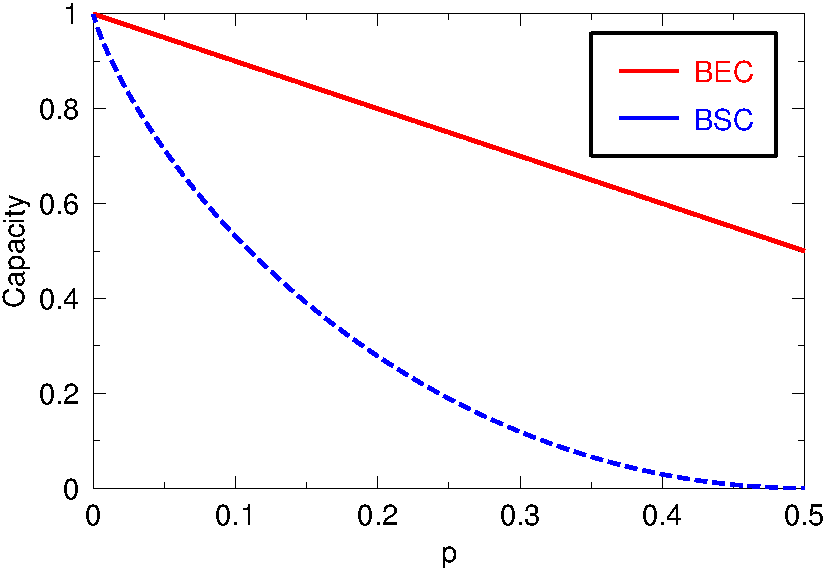
\includegraphics[width=\linewidth]{figures/becbsc.pdf}
\caption{The capacity of the BEC and BSC.}
\label{fig:becbsc}
\end{center}
\end{figure}

\booksection{Exercises}
\booksection{Further reading}
Chapter 7 in \cite{Cover_91}. 


%----------------------------------------------------------------------------------------
%	BIBLIOGRAPHY
%----------------------------------------------------------------------------------------
\chapterimage{}
\chapter*{Bibliography}
\addcontentsline{toc}{chapter}{\textcolor{ocre}{Bibliography}} % Add a Bibliography heading to the table of contents
\printbibliography[heading=bibempty]


%----------------------------------------------------------------------------------------
%	INDEX
%----------------------------------------------------------------------------------------

\cleardoublepage % Make sure the index starts on an odd (right side) page
\phantomsection
\setlength{\columnsep}{0.75cm} % Space between the 2 columns of the index
\addcontentsline{toc}{chapter}{\textcolor{ocre}{Index}} % Add an Index heading to the table of contents
\printindex % Output the index

%----------------------------------------------------------------------------------------




\end{document}
